%% uctest.tex 11/3/94
%% Copyright (C) 1988-2004 Daniel Gildea, BBF, Ethan Munson.
%
% This work may be distributed and/or modified under the
% conditions of the LaTeX Project Public License, either version 1.3
% of this license or (at your option) any later version.
% The latest version of this license is in
%   http://www.latex-project.org/lppl.txt
% and version 1.3 or later is part of all distributions of LaTeX
% version 2003/12/01 or later.
%
% This work has the LPPL maintenance status "maintained".
% 
% The Current Maintainer of this work is Daniel Gildea.

\documentclass[11pt]{ucthesis}
\def\dsp{\def\baselinestretch{2.0}\large\normalsize}
\dsp

% 2010june01 sol katzman:
% package geometry should override the various margin settings from .clo and .cls
% and also eliminates issues where the default papersize is A4
\usepackage[letterpaper, left=1.5in, right=1.25in, top=1.25in, bottom=1.25in, includefoot]{geometry}
% Use PostScript fonts as required by UCSC Dissertation Preparation Guidelines
\usepackage{pslatex}
\usepackage[utf8]{inputenc}
\usepackage{amssymb}
\usepackage{amsmath}
\usepackage{graphicx}
\usepackage{todonotes}
\usepackage{url}
\usepackage{soul}
\usepackage{xcolor}
\usepackage{xr}
\usepackage{float}
\usepackage{cite}
\usepackage[singlelinecheck=false,labelfont=bf]{caption}

\newcommand{\tool}[1]{\emph{\textsc{#1}}}

\begin{document}

% Declarations for Front Matter

\title{Graph methods for computational pangenomics}
\author{Jordan M Eizenga}
\degreeyear{2021}
\degreemonth{June}
\degree{DOCTOR OF PHILOSOPHY}
\chair{Professor Benedict Paten}
\committeememberone{Professor David Haussler}
\committeemembertwo{Professor R. Edward Green}
%\committeememberthree{Professor Ipsum Lorem}
\numberofmembers{3} %% (including chair) possible: 3, 4, 5, 6
\deanlineone{Dean Quentin Williams}
\deanlinetwo{Vice Provost and Dean of Graduate Studies}
\deanlinethree{}
\field{Bioinformatics}
\campus{Santa Cruz}

\begin{frontmatter}

\maketitle
\copyrightpage

\tableofcontents
\listoffigures
\listoftables

\begin{abstract}
Theses have elements.  Isn't that nice?
\end{abstract}

\begin{dedication}
\null\vfil
{\large
\begin{center}
To my parents,\\%\vspace{12pt}
Douglas and Lori Eizenga,\\%\vspace{12pt}
whose support is bottomless, \\\vspace{48pt}
and to my dear friend, \\%\vspace{12pt}
Corrie Janssens,\\%\vspace{12pt}
my moral North Star
\end{center}}
\vfil\null
\end{dedication}


\begin{acknowledgements}
%People to thank:
%- Benedict
%- Lab mates
%	- maybe especially Adam and Jonas
%- Friends
%- COLA and SRU
%- funding?
%- should have at least one on here that's not serious
\end{acknowledgements}

\end{frontmatter}

%side projects:
%- nanopore methylation
%- LPC
%pangenomics side projects
%- contributions to map
%- contributions to giraffe (probably leave this out)
%- review papers
%- contributions to graph L&S
%pangenomics main projects
%- my vg utilities
%	- mapq / base quality alignment
%	- sim
%	- surject
%	- autoindex
%- efficient dynamic variation graphs
%- consistent snarls
%- biclique work
%- mpmap

\part{First Part}

\chapter{Introduction and background}

%In modern genomics, sequence analysis is arguably the most fundamental experimental assay. This is in no small part due to its adaptability 

% find some breathless editorials about genomics
%The breathless tone of these popular accounts chafes the professional scientist's aesthetic of measured and dispassionate interpretation of data. The sentiment, however, rings true. 

Modern biologists can ask and answer a qualitatively greater set of questions at a quantitatively greater scale than their predecessors. Undergirding this expansion in capabilities is a deepened arsenal of technologies, and DNA sequencing is undoubtedly one of the most fundamental among them. The centrality of sequencing is due in part to the fundamental importance of DNA in biology; DNA is the (nearly) universal medium of heredity and the primary object of evolutionary change. In addition, DNA sequencing has proven to be highly adaptable for assaying various biological processes---many unbiased assays consist mainly in a method to imprint the effects of a process on DNA molecules, then followed by sequencing. 
 
% another intro: schrodinger

%TODO: this is too detailed for so early in the introduction, but i'll fix that later
%sequencing different technologies
Perhaps unsurprisingly then, many advancements in biology methodologies stem directly from advancements in sequencing technology. The problem of sequencing DNA was first solved by Frederick Sanger in 1977 by using low-frequency incorporations of a modified, chain-terminating nucleotide into synthesizing DNA molecules. The resulting shortened products could be separated using electrophoresis. Though the ``Sanger method'' served as the workhorse for early genome-sequencing projects, it has now been largely supplanted by so-called \emph{next-generation sequencing} (NGS). Although the term NGS initially encompassed several similar technologies, today the market is almost completely dominated by Illumina's platform. In this platform, synthesizing DNA molecules are terminated reversibly with a fluorophore-containing nucleotide. This allows each subsequent nucleotide to be detected using optics following a round of DNA polymerase extension. In addition, this process is massively parallel, yielding millions of short sequencing reads from a single sample. Finally, two newer \emph{third-generation sequencing} technologies, one from Pacific Biosciences (PacBio) and one from Oxford Nanopore Technologies (ONT), achieve both high throughput and long read length by sensing individual molecules rather than polymerase chain reaction (PCR) products. The cost of the longer read length is much higher error rates. Accordingly, NGS and third generation technologies currently coexist, each with their own niche of applications.

Computational methods are essential to translate sequencing data into biological insight. Often the route to biological insight involves several discrete computational steps that process the data into progressively more information-rich formats. 
%% standard genomic pipelines
%reference genomes
%genome inference
%assembly
%mapping
%variant calling




%
%RNA-seq
%spliced mapping
%expression quantification
%differential expression
%
%% technology of pipelines
%mapping 
%- indexes (k-mers hash tables, suffix array, fm-index)
%- accelerated alignment
%
%population genomics project
%- 1000 GP
%- VCF
%
%reference bias
%pangenomics
%graph genomes
%
%pangenome background
%bubbles and snarls
%string to graph alignment
%vg mapping
%variant calling

\chapter{A pantranscriptome analysis pipeline}

\section{Preamble}

What follows is the majority of the text of my preprint, "Haplotype-aware pantranscriptome analyses using spliced pangenome graphs", for which I share first-authorship with Jonas Sibbesen. The paper details three components of a pantranscriptomic pipeline. The first component builds spliced pangenome graphs, the second component aligns RNA-seq data to these graphs, and the final component infer haplotype-specific isoform analysis from the mapping results. My contributions lie primarily in the mapping algorithm and the experimental demonstrations.

\section{Introduction}

Transcriptome profiling by RNA-seq has matured into a standard and essential tool for investigating cellular state. Bioinformatics workflows for processing RNA-seq data vary, but they generally begin by comparing sequencing reads to the sequence of a reference genome or reference transcriptome \cite{li2011rsem,dobin2013star,bray2016near,patro2017salmon}. This is an expedient method that makes it practical to analyze the large volume of data produced by modern high-throughput sequencing.

Reference-based methods also have costs. When a sample's genome differs from the reference, bioinformatics tools must account for the resulting mismatches between the sequencing data and the reference. This results in reduced ability to correctly identify reads with their transcript-of-origin, with larger genomic variation leading to a greater reduction in accuracy. This problem is known as reference bias \cite{stevenson2013sources}.

Computational pangenomics has emerged as a powerful methodology for mitigating reference bias. Pangenomics approaches lean heavily on abundant, publicly-available data about common genomic variation for certain species (notably including humans). These methods incorporate population variation into the reference itself, usually in the form of a sequence graph \cite{computational2018computational,eizenga2020pangenome}. Mapping tools for pangenomic references have demonstrated reduced reference bias when mapping DNA reads \cite{garrison2018variation,rakocevic2019fast,chen2021reference}. This in turn facilitates downstream tasks that are frustrated by mapping biases, such as structural variant calling \cite{hickey2020genotyping,sibbesen2018accurate}.

The sequence graph formalism used in pangenomics has an additional attractive feature for RNA-seq data: it can represent splice junctions with little modification. Without this benefit, RNA-seq mappers for conventional references must make use of sometimes elaborate algorithmic heuristics to align over known splice junctions \cite{dobin2013star,wu2016gmap}. Alternatively, they can map to only known isoforms, but this technique has difficulty estimating mapping uncertainty due to the re-use of exons across isoforms \cite{langmead2012fast}. There is also evidence that population information can reduce reference bias problems that are particular to RNA-seq data. Accounting for population variation at splice-site motifs has been shown to aid in identifying novel splice sites \cite{stein2015discover}. 

The current methodological landscape in pangenomics is ripe to be extended to pantranscriptomics: using populations of reference transcriptomes to inform transcriptomic analyses. There is some precedent in a few existing transcriptomic methods that have used sequence graphs. \tool{AERON} \cite{rautiainen2020aeron} uses splicing graphs and \tool{GraphAligner} \cite{rautiainen2020graphaligner} to identify gene fusions. \tool{ASGAL} \cite{denti2018asgal} uses splicing graphs to identify novel splicing events. Finally, the pangenomic aligner \tool{HISAT2} \cite{kim2019graph} has its origins in the RNA-seq aligner \tool{HISAT} \cite{kim2015hisat}, and it retains many of \tool{HISAT}'s features for RNA-seq data. The performance of \tool{HISAT2} for pantranscriptomic mapping has not yet been characterized in published literature. 

One transcriptomic analysis that is particularly prone to reference bias is allele-specific expression (ASE). ASE seeks to identify differences in gene expression between the two copies of a gene in a diploid organism. These differences are indicative of various biological processes, including cis-acting transcriptional regulation, nonsense-mediated decay, and genomic imprinting \cite{zink2018insights,castel2015tools}. The differences are identified by measuring the ratio between RNA-seq reads containing each allele of a heterozygous variant. However, the reads containing the non-reference allele are systematically less mappable because of reference bias, which can lead to both degraded and illusory signals of ASE \cite{degner2009effect}. Several approaches have been developed to deal with reference bias for ASE detection. Some methods filter out biased sites \cite{van2015wasp}. Others can mitigate bias at the read mapping stage, but require variant calls, often with phasing, for the individual being analyzed \cite{rozowsky2011alleleseq,miao2018aselux,raghupathy2018hierarchical}. The variant information is either incorporated into the mapping algorithm to reduce reference bias or used to create a sample-specific diploid reference to map against. \tool{phASER} phases called genotypes using read-backed and population-based phasing to produce estimates of haplotype-specific gene expression \cite{castel2016rare}. 

Pantranscriptomic approaches using existing haplotype panels for inferring haplotype-specific expressions have also been developed. \tool{AltHapAlignR} maps reads to the linear reference genome and seven alternative HLA haplotypes to infer haplotype-specific transcript expression in the HLA region \cite{lee2018althapalignr}. \tool{HLApers} first aligns reads against all known HLA haplotypes to estimate the most likely haplotypes and then infers haplotype-specific gene expression \cite{Aguiar2019-fy}. However, both of these pantransciptomic approaches are limited to smaller genomic regions. 

In this work, we present a novel bioinformatics toolchain for whole genome pantranscriptomic analysis, which consists of additions to the vg toolkit and a new standalone tool, \tool{rpvg}. First, the \tool{vg rna} tool can combine genomic variation data and transcript annotations to construct a spliced pangenome graph. Next, \tool{vg mpmap} can align RNA-seq reads to these graphs with high accuracy. Finally, \tool{rpvg} can use the alignments produced by \tool{vg mpmap} to quantify haplotype-specific transcript expression. Moreover, the information about population variation that is embedded in the pantranscriptome reference makes it possible to do so without first characterizing the sample genome, and without restricting focus to SNVs.

\section{Results}

\begin{figure}[h!]
\begin{center}
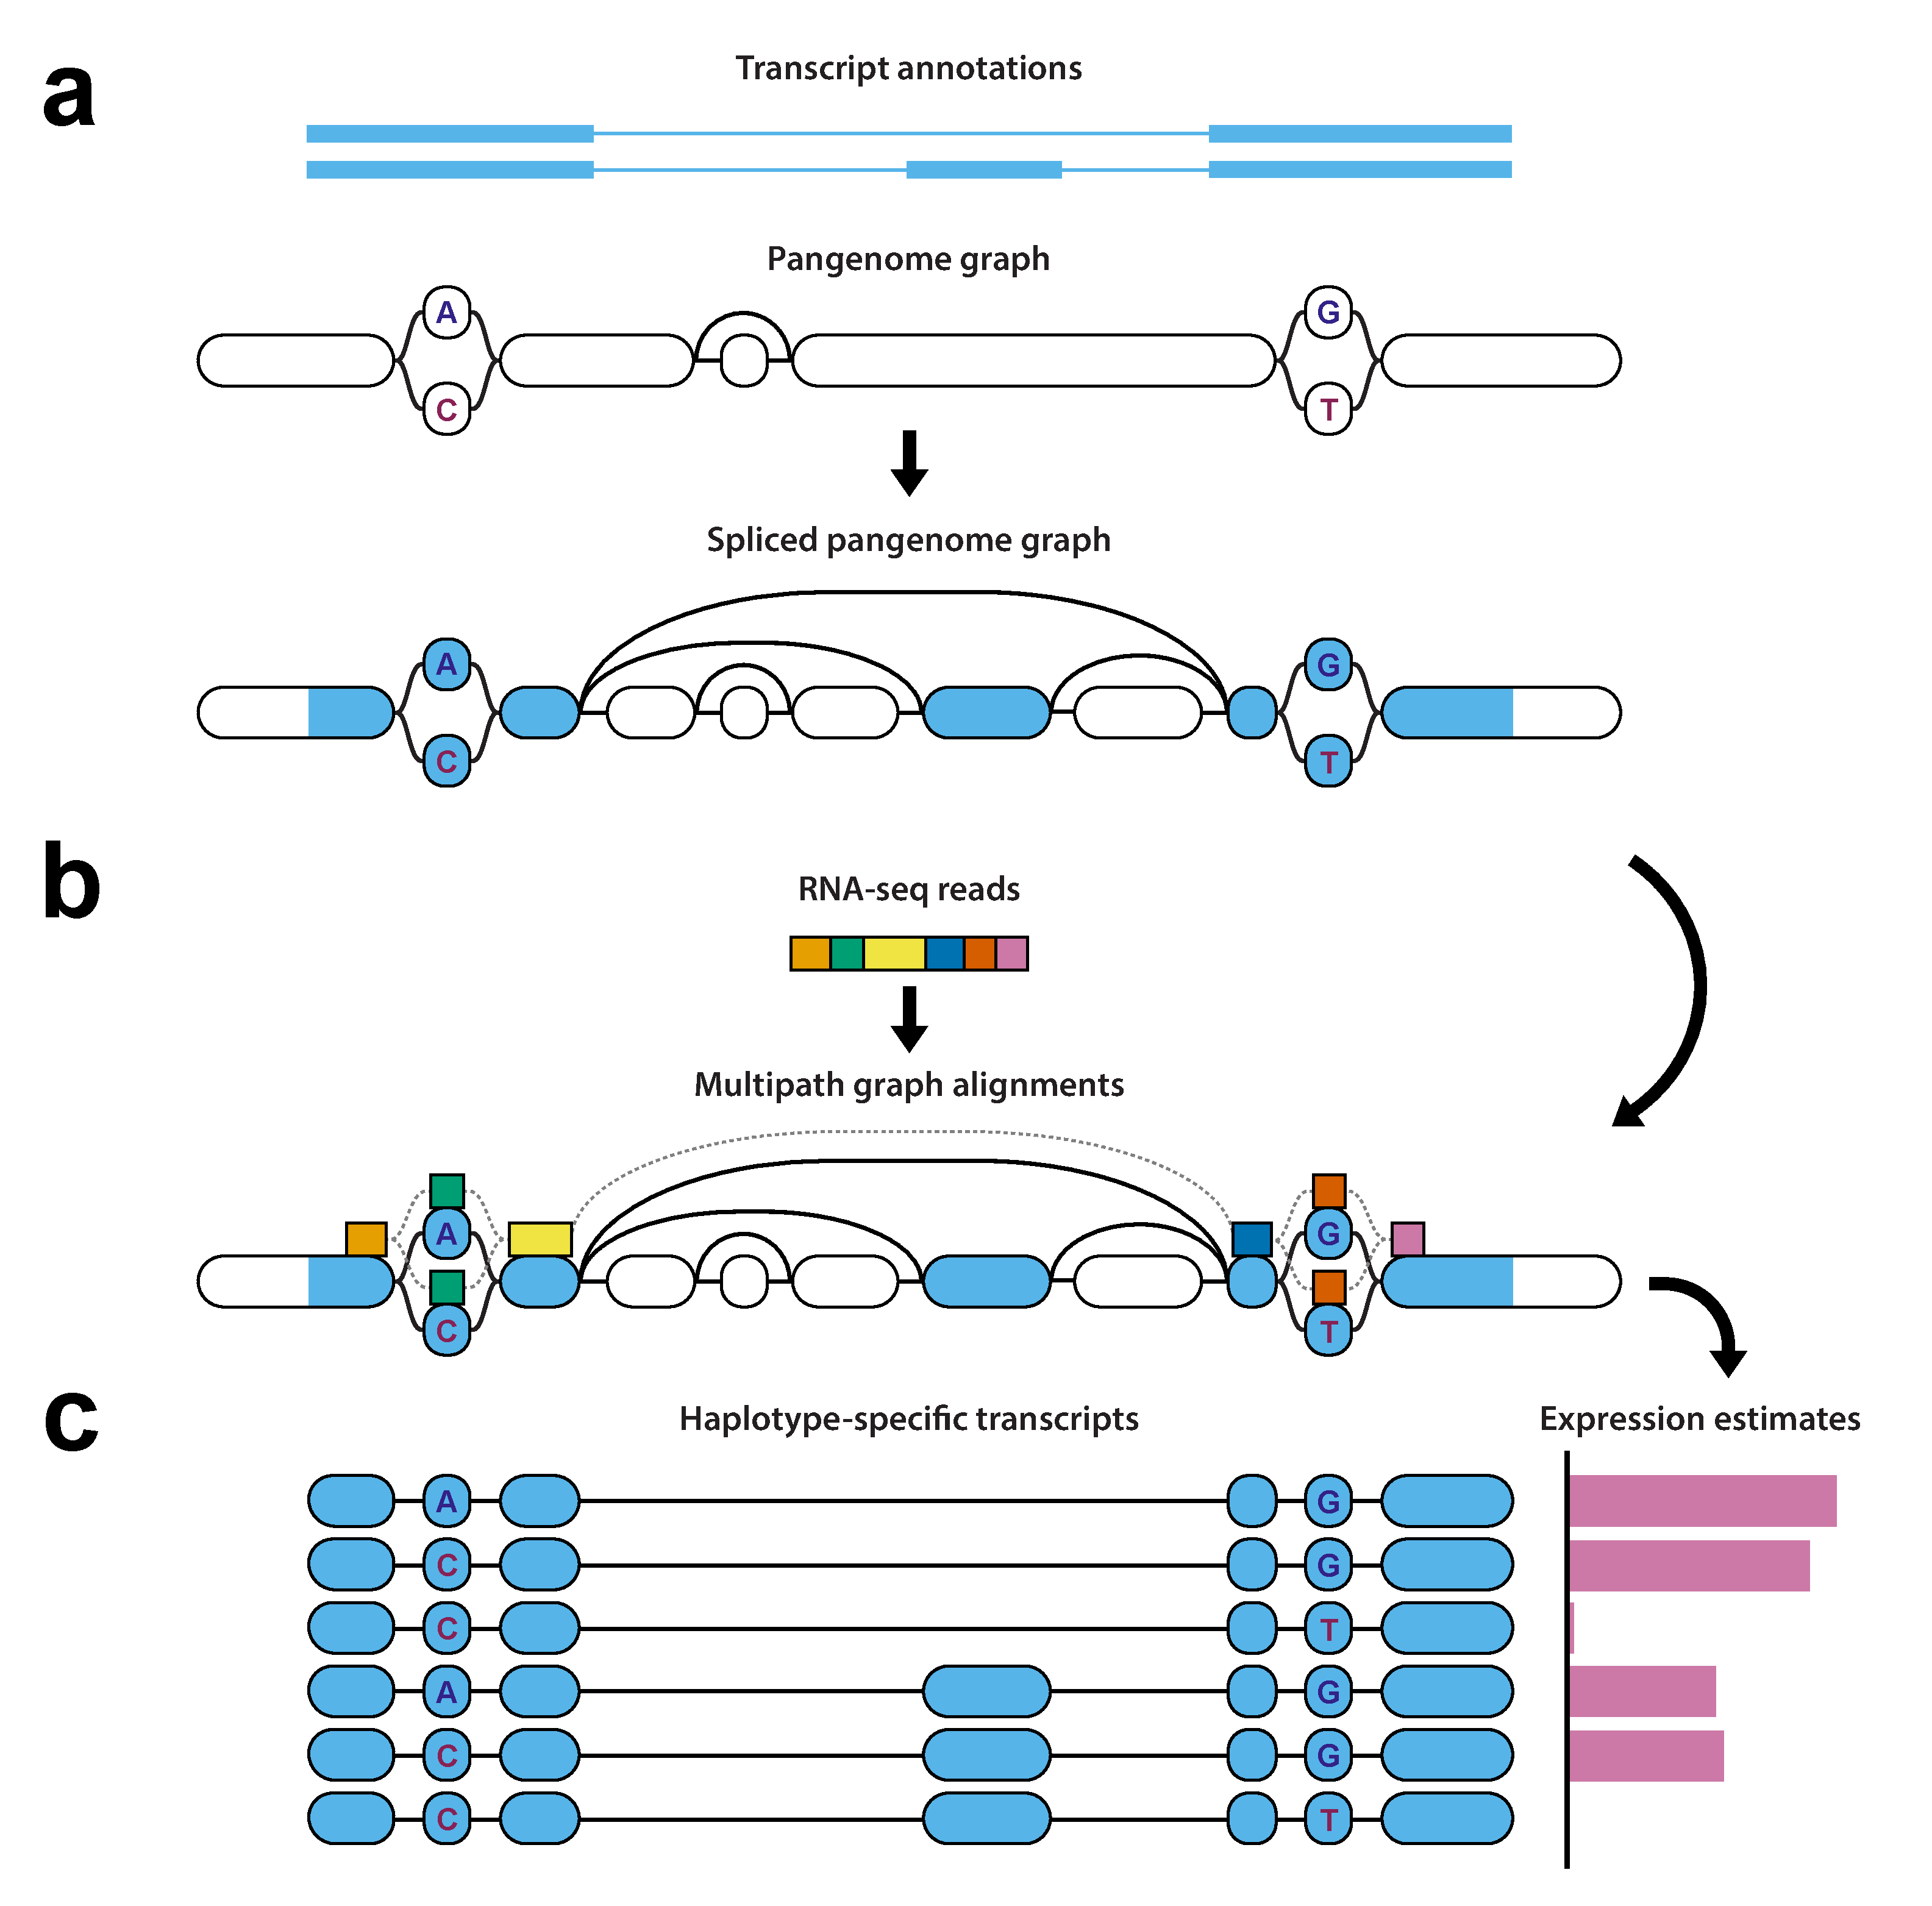
\includegraphics[width=.75\textwidth]{mpmapfigures/figure1.pdf}
\caption{\textbf{Diagram of haplotype-aware transcriptome analysis pipeline} \\
The three major steps in the pipeline. \textbf{a} \tool{vg rna} adds splice junctions derived from a transcript annotation to a pangenome graph to create a spliced pangenome graph. It simultaneously creates a pantranscriptome composed of a set of haplotype-specific transcripts (HSTs) using a panel of known haplotypes (not shown). \textbf{b} \tool{vg mpmap} aligns RNA-seq reads to subgraphs of the spliced pangenome graph represented as a multipath alignment. \textbf{c} \tool{rpvg} uses the alignments from \tool{mpmap} to estimate the expression of the HSTs in the pantranscriptome.
} \label{fig:overview}
\end{center}
\end{figure}

\subsection{Haplotype-aware transcriptome analysis pipeline}

In short, our pipeline works as follows (see Methods for a more detailed description). First, we construct a spliced pangenome graph using \tool{vg rna}, a method developed as part of the vg toolkit \cite{garrison2018variation}. \tool{vg rna} adds splice junctions from a transcript annotation into a pangenome graph as edges and then labels the paths in the graph that correspond to transcripts (Figure~\ref{fig:overview}a). Simultaneously, \tool{vg rna} constructs a set of haplotype-specific transcripts (HSTs) from the transcript annotation and a set of known haplotypes by projecting the transcript paths onto each haplotype. \tool{vg rna} uses the Graph Burrows-Wheeler Transform (GBWT) to efficiently store the HST paths allowing the pipeline to scale to a pantranscriptome with millions of transcript paths \cite{siren2020haplotype}. Next, RNA-seq reads are mapped to the spliced pangenome graph using \tool{vg mpmap}, a new splice-aware graph mapper in the vg toolkit that can align across both annotated and unannotated splice junctions (Figure~\ref{fig:overview}b). \tool{vg mpmap} produces multipath alignments that capture the local uncertainty of an alignment to different paths in the graph (Supplementary Figure~\ref{fig:multipath-alignment}). Lastly, the expression of the HSTs are inferred from the multipath alignments using \tool{rpvg} (Figure~\ref{fig:overview}c). \tool{rpvg} uses a nested inference scheme that first samples the most probable underlying haplotype combinations (e.g. diplotypes) and then infers the HST expression using expectation maximization conditioned on the sampled haplotypes.

\subsection{RNA-seq mapping benchmark}

We compared \tool{vg mpmap} against three other mappers: \tool{STAR} \cite{dobin2013star}, \tool{HISAT2} \cite{kim2019graph} and \tool{vg map} \cite{garrison2018variation}. \tool{STAR} and \tool{HISAT2} can both use splicing information to guide mapping, but of the two only \tool{HISAT2} is able to also utilize genomic variants. \tool{vg map} is not a splice-aware mapper, but it is still able to map to spliced pangenome graphs, which contain both splicing and genomic variation edges. 

We used two different references for the comparison: the standard reference genome with added splice junctions (spliced reference) and a spliced pangenome graph containing both splice junctions and variants (spliced pangenome graph). For \tool{STAR} only the spliced reference was used. 

\begin{figure}[h!]
\begin{center}
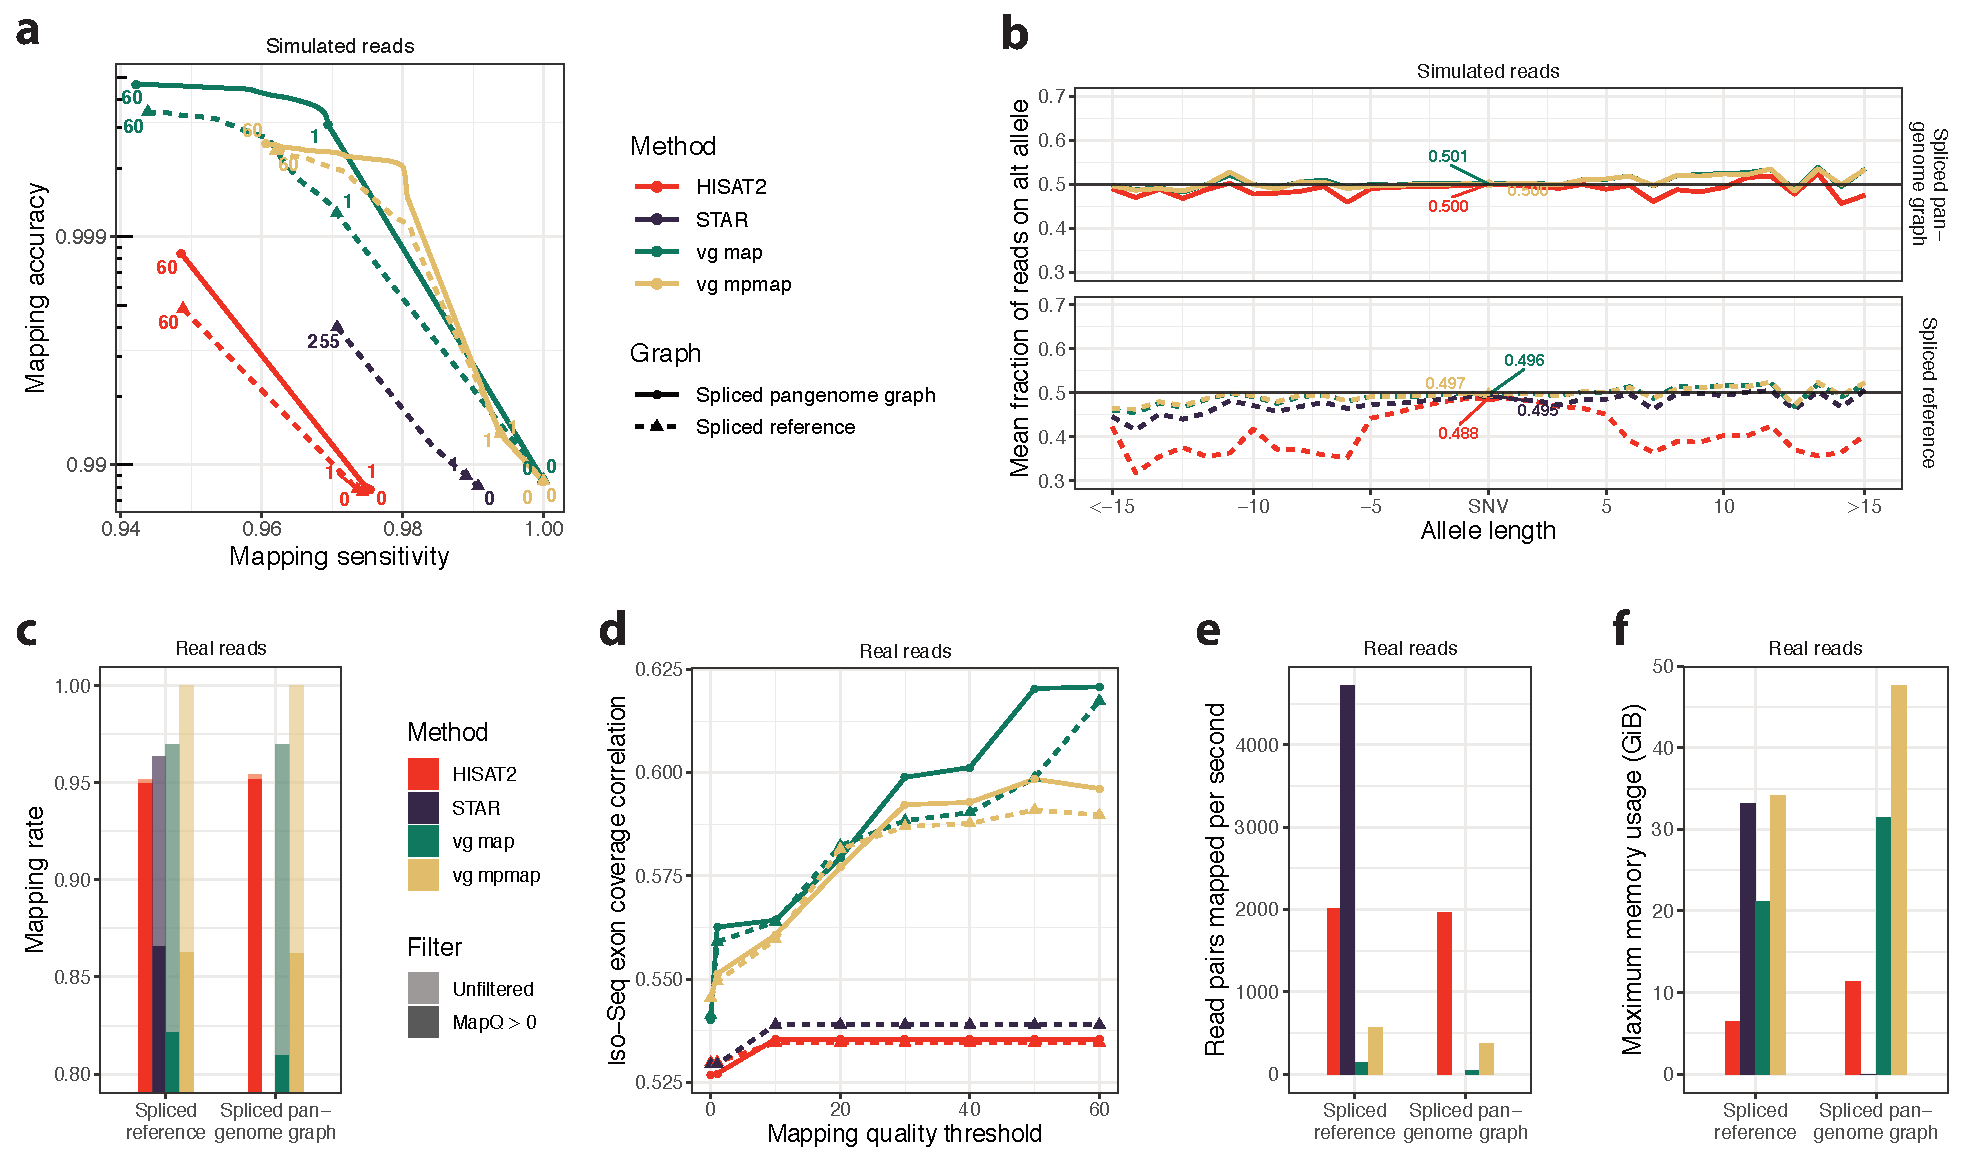
\includegraphics[width=\textwidth]{mpmapfigures/figure2.pdf}
\caption{\textbf{Mapping benchmark using RNA-seq data from NA12878} \\
RNA-seq mapping results comparing \tool{vg mpmap} and three other methods using simulated and real Illumina data (``vg sim (ENC, uniform)'' and ``ENCSR000AED'' in Supplementary Table~\ref{tab:sim-data} and~\ref{tab:read-sets}, respectively). Solid and dashed lines show the results using a spliced pangenome graph and spliced reference, respectively. \textbf{a} Mapping accuracy and sensitivity for different mapping quality thresholds (colored numbers) using simulated data. An alignment is considered correct if it covers 90\% of the true reference sequence alignment. \textbf{b} Mean fraction of mapped reads supporting the non-reference allele for variants of different lengths in simulated data. Negative lengths correspond to deletions and positive to insertions. The colored numbers are the mean fraction for SNVs. \textbf{c} Mapping rate using real data. The shaded bars show the mapping rate for all alignments and the solid bars for only alignments with a mapping quality above 0. \textbf{d} Pearson correlation between Illumina and Iso-Seq exon coverage using real data as a function of mapping quality threshold. Exons are defined by the Iso-Seq alignments. \textbf{e} Number of read pairs mapped per second per thread using real data. The mapping times were estimated using 16 threads on a AWS m5.4xlarge instance. \textbf{f} Maximum memory usage for mapping in gigabytes using real data.  
} \label{fig:mapping}
\end{center}
\end{figure}

\subsubsection{Simulated sequencing data}

Paired-end reads were simulated from HSTs derived from the GENCODE transcript annotation set \cite{frankish2019gencode} and the NA12878 haplotypes from the 1000 Genomes Project (1000GP) \cite{10002015global}. \tool{vg sim} was used to simulate the reads using reads from the ENCODE project (ENCSR000AED replicate 1) to parameterize the noise model \cite{encode2012integrated,davis2017encycolopedia}. Fragment length distribution parameters used in the simulation were estimated from the same reads using \tool{RSEM} \cite{li2011rsem}. The CEU population was excluded from the spliced pangenome graph as NA12878 is from that population, and we wanted to estimate performance for a new individual, who may not be as closely-related to the 1000GP populations. We simulated the HSTs with uniform expression rather than trying to match a previous expression profile, which could bias expression towards easily-mappable transcripts. 
\newline 
\newline 
Using the set of simulated reads we first compared the overall mapping performance of each method. Figure~\ref{fig:mapping}a shows the mapping sensitivity and accuracy (log-scale) for different mapping quality thresholds. An alignment was considered correct if it covered 90\% of the true reference sequence alignment. The graph alignments from \tool{vg map} and \tool{vg mpmap} were projected to the reference sequence for this comparison. As can be seen in Figure~\ref{fig:mapping}a, \tool{vg mpmap} achieves both a high sensitivity and accuracy, while the other methods either had a lower accuracy or sensitivity. The results also show that the spliced pangenome graph generally improves mapping performance. 

To evaluate the method's ability to align over unannotated splice junctions, we repeated the experiment on a spliced pangenome graph (spliced reference for \tool{STAR}) created from an annotation set with 20\% of the transcripts missing (Supplementary Figure~\ref{fig:splice-junction-mapping}). This number was based on recent estimates of the fraction of novel transcripts in a sample using long reads \cite{wyman2019technology}. As expected, the performance of \tool{vg map} decreases dramatically since it can only align over splice junctions represented in the graph. \tool{vg mpmap}'s performance decreased markedly more on the downsampled annotation compared to \tool{STAR} and \tool{HISAT2} using the 90\% threshold (Supplementary Figure~\ref{fig:splice-junction-mapping}a). This is likely due to its more conservative approach to finding novel splice-junctions that require a high-scoring alignment in order for a new junction to be statistically significant. Indeed, when using a threshold of 70\%, the mapping accuracy \tool{vg mpmap} increases to a value higher than \tool{STAR} and \tool{HISAT2} even when they use the complete transcript set (Supplementary Figure~\ref{fig:splice-junction-mapping}b).

Next, we looked at whether using a variant-aware approach reduces reference bias. Figure~\ref{fig:mapping}b shows the mean fraction of reads mapped to the alternative allele for different allele lengths. Negative values correspond to deletions and positive values to insertions. When using the spliced reference genome, all methods exhibit a bias towards the reference allele, with \tool{vg map} and \tool{mpmap} showing less bias than the other methods. Using the spliced pangenome graph results in substantially reduced bias for all 
methods.

The mapping results were corroborated by an alternate correctness criterion based on aligning within 100 bases of the correct position on the paths in the graph (Supplementary Figure~\ref{fig:mapping-gampcompare}).
\newline 
\newline
The set of simulated reads used for the mapping evaluation was not used to optimize the development and parameters of \tool{vg map} and \tool{mpmap}. Supplementary Figure~\ref{fig:mapping-srr}a shows the results on the dataset that was used for optimization, which used RNA-seq data from Tilgner et al. \cite{tilgner2014defining} to parameterize the read simulation. The sensitivity and accuracy estimates for \tool{mpmap} are quite similar between the two datasets indicating that \tool{mpmap} is not overfit to the training data. The performance of all the other methods was generally worse on the training data. 

\subsubsection{Real sequencing data}

We used the same read set from the ENCODE project that was used to parametrize the simulations to benchmark the methods on real data. We first looked at the fraction of aligned reads for each method (Figure~\ref{fig:mapping}c). \tool{vg mpmap} was able to map more reads overall than any of the other methods. \tool{HISAT2} achieved a higher mapping rate for mappings with mapping quality greater than 0, but seemingly at the cost of low specificity (Figure~\ref{fig:mapping}a). Using the spliced pangenome graph did not have a notable influence on the mapping rates. 

Ground-truth alignments are not available for real data, so we use a proxy based on Pacific Biosciences (PacBio) Iso-Seq read mappings instead. Specifically, we compare to Iso-Seq read alignments generated by the ENCODE project (ENCSR706ANY) from the same cell line as the Illumina reads. Since the cell line is the same, we expect the transcript expression to be similar. Moreover, long reads can generally be mapped more confidently than short reads. Thus, higher correlation in coverage between short read mappings and the Iso-Seq mappings should be indicative of more accurate short read mappings in the aggregate. Figure~\ref{fig:mapping}d shows the estimated Pearson correlation in the coverage of each exon as a function of mapping quality threshold. As can be seen, both \tool{vg map} and \tool{mpmap} achieves higher correlation than \tool{STAR} and \tool{HISAT2}, with the spliced pangenome graph resulting in even higher correlation for both. The graph alignments from \tool{vg map} and \tool{mpmap} were projected to the reference genome for this analysis.  

Finally, we compared the methods' mapping speed and memory usage. Figure~\ref{fig:mapping}e shows the number of read pairs mapped per second per thread. Conversion from SAM to BAM was included in the \tool{HISAT2} time estimate to be more comparable to the output type of the other methods. \tool{vg mpmap}'s increase in accuracy does not come for free; it is between 3.6 and 5.2 times slower than \tool{HISAT2}, depending on the graph. However, it is 9.4 times faster than \tool{vg map} on the spliced pangenome graph. \tool{vg mpmap} uses slightly more memory than \tool{STAR} (Figure~\ref{fig:mapping}f). 
\newline 
\newline
We also compared the mapping performance of the different methods on the real RNA-seq data from Tilgner et al. \cite{tilgner2014defining} and CHM13 RNA-seq data from the T2T consortium (Supplementary Figure~\ref{fig:mapping-srr}b,c and~\ref{fig:mapping-t2t}). Similar overall tendencies are observed using these datasets. It is important to mention that the CHM13 data was used during the development of \tool{vg mpmap}, and the other set was used to optimize the parameters of \tool{vg map} and \tool{vg mpmap}.

\subsection{Haplotype-specific transcript quantification}

\begin{figure}[h!]
\begin{center}
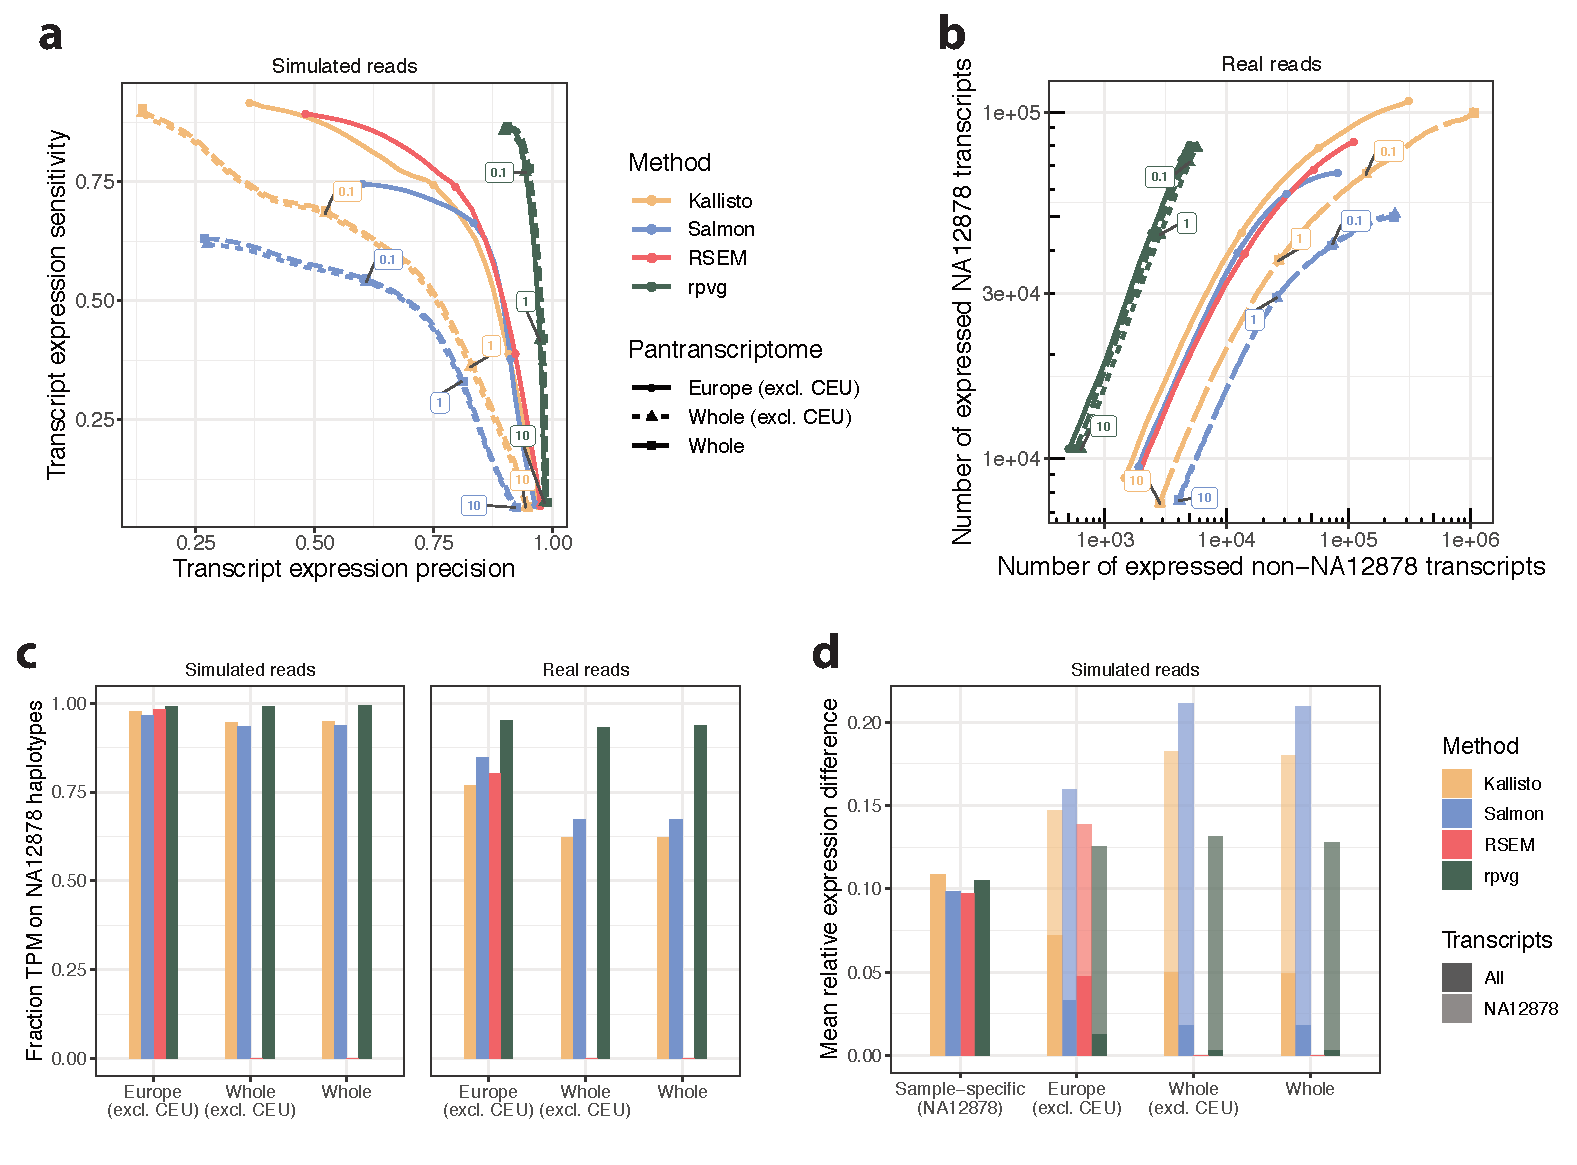
\includegraphics[width=.85\textwidth]{mpmapfigures/figure3.pdf}
\caption{\textbf{Haplotype-specific transcript quantification benchmark using RNA-seq data from NA12878} \\
Haplotype-specific transcript (HST) quantification results comparing \tool{rpvg} against three other methods using simulated and real Illumina data (``vg sim (ENC, RSEM)'' and ``ENCSR000AED'' in Supplementary Table~\ref{tab:sim-data} and~\ref{tab:read-sets}, respectively). Solid lines with circles are results using a pantranscriptome generated from 1000 Genomes Project (1000GP) European haplotypes excluding the CEU population. Dashed lines with triangles and squares are results using a pantranscriptome generated from all 1000GP haplotypes without and with the CEU population, respectively. \textbf{a} Sensitivity and precision of whether a transcript is correctly assigned nonzero expression for different expression value thresholds (colored numbers for ``Whole (excl. CEU)'' pantranscriptome) using simulated data. Expression is measured in transcripts per million (TPM). \textbf{b} Number of expressed transcripts from NA12878 haplotypes shown against the number from non-NA12878 haplotypes for different expression value thresholds (colored numbers) using real data. \textbf{c} Fraction of transcript expression (in TPM) assigned to NA12878 haplotypes for different pantranscriptomes using simulated (left) and real (right) data. \textbf{d} Mean absolute relative difference (MARD) between simulated and estimated expression (in TPM) for different pantranscriptomes using simulated data. MARD was calculated using either all HSTs in the pantranscriptome (solid bars) or using only the NA12878 HSTs (shaded bars). ``Sample-specific (NA12878)'' is a personal transcriptome generated from 1000GP NA12878 haplotypes.  
} \label{fig:expression}
\end{center}
\end{figure}

We compared \tool{rpvg} to three other transcript quantification methods: \tool{Kallisto} \cite{bray2016near}, \tool{Salmon} \cite{patro2017salmon} and \tool{RSEM} \cite{li2011rsem}. We stress that none of these methods were developed to work on pantranscriptomes with millions of HSTs. However, they serve as a point of reference for what accuracy is achievable without new methods development. The simulated data was generated by \tool{vg sim}, largely as described for the mapping benchmark. The only difference was that, rather than simulating transcripts with uniform expression, we simulated according to an expression profile that was estimated by \tool{RSEM} using the same ENCODE reads. Three different pantranscriptomes were generated for the evaluation using different sets of 1000GP haplotypes (Supplementary Table~\ref{tab:pantranscriptomes}): 1) all European haplotypes excluding the CEU population (Europe (excl. CEU)) 2) all haplotypes excluding the CEU population (Whole (excl. CEU)) and 3) all haplotypes (Whole). The CEU population was excluded for the same reason as in the mapping benchmark: because NA12878 is part of this population, and we wanted to evaluate the realistic setting in which a sample is not as well represented by the haplotype panel. In addition, we created a sample-specific transcriptome consisting of NA12878 HSTs (Sample-specific (NA12878)). This transcriptome corresponds to the ideal case where a sample's haplotypes are known beforehand. 
\newline 
\newline
We first looked at the method's ability to accurately predict whether an HST was correctly expressed or not. Figure~\ref{fig:expression}a shows the sensitivity and precision of whether a transcript is correctly expressed or not using simulated data. The results were stratified by different expression thresholds up to a value of 10 TPM (transcripts per million). Note that we were not able to run \tool{RSEM} on the two largest pan-transcriptomes used in the figure. \tool{rpvg} exhibits a mucher higher precision and sensitivity than the other tools for all pantranscriptomes. Over 97.4\% of the HSTs with an expression value of at least 1 TPM are correctly predicted to be expressed by \tool{rpvg} using the ``Whole (excl. CEU)'' pantranscriptome. Importantly, only a minor difference is observed between the pantranscriptomes without the CEU population (excl. CEU) and the whole pantranscriptome (Whole), which contains NA12878. This could be explained by the fact that less than 2\% of HSTs are on average unique to a specific sample when compared to all samples in other populations using the 1000GP data (Supplementary Figure~\ref{fig:hst-populations}). This suggests that haplotype panels like the 1000GP are a good alternative when a sample's haplotypes are not available, although there are always limits to panel diversity, and some samples will be less well-represented by a 1000GP pantranscriptome. 

We also evaluated the accuracy of the HST expression estimation using real sequencing data (Figure~\ref{fig:expression}b). Since we do not know which transcripts are expressed in real data, we focus instead on the haplotype estimation. Sample NA12878's haplotypes are known to a reasonably high degree of certainty. Thus, we can indirectly measure accuracy by asking whether the HSTs that are estimated to be expressed are in fact from NA12878. Similar to the simulated data, Figure~\ref{fig:expression}b shows that \tool{rpvg} predicts markedly fewer HSTs from non-NA12878 haplotypes than both \tool{Kallisto} and \tool{Salmon}. Using the ``Whole (excl. CEU)'' pantranscriptome, \tool{rpvg} predicted 2,836 HSTs from non-NA12878 haplotypes to have an expression value of at least 1 TPM, while \tool{Salmon} and \tool{Kallisto} predicted 25,790 and 26,779, respectively. 

Next, we compared the fraction of transcript expression (in TPM) that was attributed to NA12878 haplotypes. This is shown in Figure~\ref{fig:expression}c for both simulated (left bars) and real (right bars) data. We see that \tool{rpvg} attributes more than 98.9\% and 93.1\% of the expression to NA12878 haplotypes when using simulated and real data, respectively. Furthermore, the figure shows that \tool{rpvg}'s prediction accuracy only decreases slightly when the size of the pantranscriptome increases from 2.5M HSTs in ``Europe (excl. CEU)'' to 11.6M in ``Whole (excl. CEU)''.  
\newline 
\newline
We compared how well the different methods could predict the correct expression value. Figure~\ref{fig:expression}d shows the mean absolute relative difference (MARD) between the expression values of the simulated reads and the estimated values. The solid bars are MARD values when using all HSTs in the pantranscriptomes, and the shaded bars are when comparing the NA12878 HSTs only. Note that these bars are the same for the sample-specific set, which consists of only NA12878's HSTs. On the sample-specific set, \tool{rpvg} performs comparably to the other methods. However, as the size of the pantranscriptome grows, the increase in MARD on the NA12878 transcript set is considerably less for \tool{rpvg} relative to the other methods. When looking at the whole transcript set in each pantranscriptome (solid bars), \tool{rpvg} has the lowest MARD. The much lower values compared to the NA12878 transcript set can be explained by the large number of unexpressed HSTs in the full pantranscriptomes.

We also compared the expression values using Spearman correlation (Supplementary Figure~\ref{fig:expression-corr}). This metric supported overall similar conclusions, albeit with \tool{Kallisto} and \tool{RSEM} performing comparably to \tool{rpvg} when using the pantranscriptomes but restricting focus to NA12878's haplotypes. This suggests that \tool{Kallisto} and \tool{RSEM} accurately rank these transcripts' expression but do not accurately estimate the absolute quantity.
\newline 
\newline
To show the advantage of the multipath alignment format when inferring HST expression we repeated the evaluation using single-path alignments as input to \tool{rpvg} (Supplementary Figure~\ref{fig:expression-multipath}). The single-path alignments were created by finding the best scoring path in each multipath alignment. For all pantranscriptomes and datasets, \tool{rpvg} gave the best results using the multipath alignments.

Similarly to the mapping benchmark, we also evaluated \tool{rpvg} on RNA-seq data from the CHM13 cell line and NA12878 RNA-seq data from Tilgner et al. \cite{tilgner2014defining} (Supplementary Figure~\ref{fig:expression-t2t} and~\ref{fig:expression-srr}). Overall, similar conclusions can be drawn using these data. It is important to mention that both datasets were used to optimize the parameters of \tool{rpvg}.

\section{Discussion}

The pace of development in the field of eukaryotic pangenomics has surged in recent years. Improvements in sequencing technology have made it practical to characterize the genomes of increasingly many samples. As a result, pangenomes made from tens to hundreds of reference-quality genome assemblies have been constructed for several agricultural organisms \cite{jayakodi2020barley,crysnanto2019accurate,liu2020pan}, and similar efforts are underway for humans by the Human Pangenome Reference Consortium and others \cite{ebert2021haplotype}. Simultaneously, the bioinformatics tools to do pangenomic analyses have matured to the point of practicality for many applications \cite{manuweera2019pangenome,hickey2020genotyping,siren2020genotyping}. Moving forward, we anticipate that pangenomic methods will continue to expand to inform increasingly many areas of genomics \cite{groza2020personalized}.

In this work, we have presented one step in this expansion: generalizing transcriptomics into pantranscriptomics. Our novel bioinformatics pipeline provides a full stack of tools for pantranscriptomic analysis. It can construct pantranscriptomes, map RNA-seq reads to these pantranscriptomes, and quantify transcription with haplotype-resolution. The construction takes advantage of efficient pangenome data structures, the mapping achieves a desirable balance of accuracy and speed, and the quantification can infer haplotype-specific transcript expression even when the sample's haplotypes are not known beforehand.

Some downstream use cases are already apparent. This pipeline can be used to characterize genotypes and haplotypes in coding regions from RNA-seq data, giving access to the exact transcript sequences in a sample's transcriptome. It also can be used to study causes of haplotype-specific expression, such as imprinting, nonsense-mediated decay, and cis-regulation. In both cases, this pipeline increases the information that is available from RNA-seq data without paired genomic sequencing. This will enable low-cost study designs and deeper reanalyses of existing data.

Of course, our pipeline also has limitations. We have developed it to have good performance on pantranscriptomes constructed from phased variant calls. This is presently the most available data resource for constructing pangenomes. However, as increasingly many haplotype-resolved assemblies are produced, we predict that the emphasis in pangenomics will shift to pangenome graphs constructed from whole genome alignments. Constructing these graphs is currently an area of active research \cite{li2020design,jandrasits2018seq}. Such graphs have more complicated topologies, often involving complex cyclic motifs. Experience leads us to believe that pantranscriptomic tools will require further methods development to use these data resources effectively.

Our pipeline is optimized for short-read RNA-seq data. The higher-error long-read RNA-seq technologies developed more recently require specifically-tailored algorithms for efficient analysis \cite{li2018minimap2,wyman2019technology}. Pantranscriptomic analyses of long-read RNA-seq data will likewise require further development, although the pipeline described here could serve as a platform for this development. Nevertheless, the cost-effectiveness of short-read sequencing virtually ensures that it will remain an important part of the sequencing landscape into the near future.

Our pipeline also relies on having a comprehensive pantranscriptome that contains many of the sample's haplotype-specific transcripts. The pantranscriptomes used in this study (based on the 1000 Genome Project) provided good results in the two samples analyzed, but this performance may not extend to samples from other populations. Here?and throughout pangenomics?there is a compelling case to improve the completeness of data resources through more diverse sampling.

%%%%%%%%%%% Comment thread imported from Google doc %%%%%%%%%%%%%%%
% Benedict: Might also be worth mentioning single-cell applications. e.g. Imagine trying to quantify somatic haplotype-specific expression in subsets of tumor cells? I appreciate this is a bit science fiction now, but perhaps not for too much longer.
% Jordan: I don't think I totally understand this use case, tbh. What's the edge we get from bringing a pantranscriptomic methodology?
% Benedict: sorry, totally half baked, but what I was thinking vaguely was that if you could build tumor-specific transcripts from dna sequencing of a tumor you could use the approach to quantify tumor-haplotype specific expression? again, half baked.
% Jordan: Hmm. We could probably do that analysis with mpmap/rpvg, but it seems to me the harder part would be the DNA sequencing. You'd need to produce something like a phased "tumor pangenome", and you'd have to do the phasing without even the benefit of assuming unbiased coverage of 2 haplotypes (because the fraction of clonal populations differs).
% Jonas: One thing we could try is to use mpmap/rpvg to infer the germline haplotypes and quantify the expression of germline haplotype-specific transcripts in a cancer RNA-seq sample. This could maybe then be used as a "background" for downstream somatic variant/expression analyses (haven't thought this through thoroughly yet). I think this might be doable with the pipeline already assuming that somatic variation are different from the variants in the pantranscriptome (which I think is a fair assumption). I have no idea how mpmap/\tool{rpvg} will perform on this data, but it could be interesting to explore this maybe as part of the use-case figure.
% Jordan: I think that's reasonable but also comfortably fits under the umbrella of the "low cost study designs and deeper reanalyses" that we already mention, since the mpmap/\tool{rpvg} portion would basically just be treating the scRNA-seq as bulk sequencing. Is the goal here just to mention a single cell application? If so, I think it would be less of a stretch to focus on random mono-allelic expression in somatic tissues. That's an analysis that we would actually need single cell sequencing for.

\section{Acknowledgements}

Research reported in this publication was supported by the National Human Genome Research Institute of the National Institutes of Health under Award Numbers U01HG010961 and R01HG010485. The content is solely the responsibility of the authors and does not necessarily represent the official views of the National Institutes of Health. The work of JAS was supported by the Carlsberg Foundation. We thank the ENCODE Consortium, the Thomas Gingeras Laboratory (Cold Spring Harbor Laboratory) and the Ali Mortazavi Laboratory (University of California Irvine) for generating and sharing the ENCODE data used in this study. We would also like to thank Megan Dennis (University of California Davis) for generating and providing access to the CHM13 RNA-seq data on behalf of the T2T consortium. Finally, we would like to thank Jean Monlong and Glenn Hickey for feedback on the manuscript, and everybody else in the vg team.

\section{Methods}

\subsection{Sequencing data, transcript annotations and variation databases}

GENCODE v29 (primary assembly) was used as a transcript annotation set \cite{frankish2019gencode}. All transcripts with either the mRNA\_start\_NF or mRNA\_end\_NF tag were removed in order to only keep confirmed full-length transcripts. Furthermore, a transcript subset containing 80\% of the GENCODE transcripts was created by randomly removing 34,490 of the 172,449 transcripts in the annotation. The fraction removed was based on recent estimates of the fraction of novel transcripts in a sample using long reads \cite{wyman2019technology}.

Genomic variants on GRCh38 from the 1000 Genomes Project (1000GP) were downloaded from EBI (\url{http://ftp.1000genomes.ebi.ac.uk/vol1/ftp/release/20130502/supporting/GRCh38_positions/}) \cite{10002015global}. The variants were first normalized using \tool{bcftools} \cite{Li2011-xc} and four different sets containing variants from differently-sized collections  of samples were created (Supplementary Table~\ref{tab:haplotype-sets}). Two of these sets were constructed so as to not include variants unique to the CEU population. This was because we benchmarked the pipeline on NA12878, who is from this population, and we wanted our evaluations to cover one of the intended use-cases for the pipeline: sequencing a new sample from a population that is not represented in the reference haplotype panel. For all of the variant sets except the sample-specific set (where allele frequency was not relevant), the intronic and intergenic variants were further filtered using \tool{bcftools}, keeping only variants with an alternative allele frequency of at least 0.002 or 0.001 depending on the set. This was done to decrease the complexity of the graph in regions where fewer reads are expected to map. The GRCh38 (primary assembly) reference genome used throughout the study was downloaded from Ensembl (\url{ftp://ftp.ensembl.org/pub/release-94/fasta/homo_sapiens/dna/}).  
\newline 
\newline
A list of all sequencing data used can be found in Supplementary Table~\ref{tab:read-sets}. 

\subsection{Spliced pangenome graph construction}

We developed a method in the vg toolkit, \tool{vg rna}, for constructing spliced pangenome graphs from a transcript annotation and an existing pangenome graph. \tool{vg rna} begins by identifying the path in the graph that corresponds to each exon in the annotation. This process is facilitated by indexes in the vg toolkit that can efficiently query graph locations of positions on the linear reference. These exon paths can start or end internally in a node rather than only at boundaries between nodes, as with other paths in vg. Next, \tool{vg rna} divides nodes as necessary to expose exon boundaries as node boundaries and then adds edges (splice-junctions) to the graph connecting adjacent exons within each transcript. The transcript paths are then labeled in the resulting spliced pangenome graph. Lastly, the spliced pangenome graph's node ID space is compacted and reordered in topological order to make graph compression more efficient \cite{eizenga2020efficient}. 
\newline 
\newline
In addition to the spliced pangenome graphs, \tool{vg rna} was also used to construct exon-only splicing graphs. \tool{vg rna} creates these graphs by removing all nodes and edges from a spliced pangenome graph that were not covered by a transcript path. Different combinations of transcript annotations (full and an 80\% random subset) and variant sets (Supplementary Table~\ref{tab:haplotype-sets}) were used as input to create the graphs used in the mapping and expression inference evaluation. 

\subsection{Pantranscriptome construction}

In addition to constructing spliced pangenome graphs, \tool{vg rna} can simultaneously generate pantranscriptomes consisting of haplotype-specific transcripts (HSTs) created from transcript and haplotype annotations. It creates pantranscriptomes by projecting the reference transcript paths onto haplotypes paths that are either labeled in the graph or indexed using the Graph Burrows-Wheeler transform (GBWT) \cite{siren2020haplotype}. The GBWT is a succinct data structure for efficiently storing thousands of paths in a graph, such as haplotypes or transcripts. If nodes are split during the spliced pangenome graph construction (see above), \tool{vg rna} first updates the haplotypes in the input GBWT. Next, the flanking positions of the exon boundaries on the reference chromosome path are located in the graph. These positions are used as anchors for projecting exons between the reference and haplotype paths. Anchoring on the positions adjacent to exon boundaries allows for genomic variation at the distal ends of exons. 

Depending on whether the haplotype paths are labeled in the graph or stored in a GBWT, the projection is performed differently. For haplotype paths that have been labeled in the graph, we first locate all paths that contain both anchor nodes for each exon in a transcript. Next, for each located exon anchor pair we then follow the haplotype path between the two anchors to create the projected haplotype-specific (HS) exon path. HST paths are then created by combining all HS exon paths that are projected to the same haplotype. Only complete transcripts where all exons are successfully projected are kept. A projection will fail if there is variation at the anchor position in the target haplotype. Finally, HST transcripts that are identical are collapsed, producing a set of unique HSTs for each reference transcript. Since the number of pre-collapsed HSTs can be as large as the number of haplotypes, the algorithm is not suitable for large haplotype sets. For these, the GBWT-based algorithm, described below, is a better choice.

% \todo{Adam: Should this be "will fail"? Or are some but not all types of variation tolerated? And if so, which ones are acceptable and which cause the projection to fail? Jonas: Yes, good point. It should be will.}

A broadly similar approach is used when the haplotype paths are stored in a GBWT. However, it differs in how the projected exons paths are constructed and combined. To find all possible haplotype paths between two exon anchors, we use a depth-first search (DFS). The search is initialized at the start anchor and traverses all possible paths in the graph starting from that anchor. Each explored exon path in the DFS (branch) is queried against the GBWT index and is terminated if it is not a subpath of any haplotypes in the index. Furthermore, a branch is also terminated if it is not possible to reach the end anchor node by any of the haplotypes consistent with the exon path. This is determined by examining whether any of the haplotypes containing the exon path also contain the end anchor node. The output from the search is a list of unique projected HS exon paths and the set of haplotypes consistent with each of them. The final HST paths are constructed one exon at a time by connecting HS exon paths that share at least one haplotype for each transcript. Because all the HS exon paths are unique this procedure will always result in a set of only unique HST paths and thus it is not necessary to collapse identical paths. This attribute makes the approach using the GBWT scale well with the number of haplotypes, as it can take advantage of the fact that haplotypes are often identical locally.
\newline 
\newline
A list of all pantranscriptomes created for this study including the transcript annotations and variant sets used as input can be seen in Supplementary Table~\ref{tab:pantranscriptomes}. The HSTs were written both as nucleotide sequences in FASTA format and as paths to a GBWT. A bidirectional GBWT, where each path is stored in both directions, was also created. \tool{rpvg} uses this index to decrease computation time when reads are not strand-specific. For each GBWT, a corresponding $r$-index was further constructed. This index, based on the original $r$-index by Gagie et al., significantly decreases the computation time it takes to query path IDs in the GBWT \cite{Gagie2020-lq}.

\subsection{Read simulation model}

Simulated reads were generated using \tool{vg sim}, a read simulator in the vg toolkit that is designed primarily for next-generation sequencing (NGS) reads. Its model consists of three components: a Markov model for base quality strings, a path frequency model, and a fragment length model (when sampling paired-end reads).

The model for base quality strings is fit to replicate the base quality strings in a user-provided FASTQ. A separate Markov transition distribution is fit for each base position in the read. The state of each Markov distribution consists of two components: the Phred base quality at that base and whether that base is an N. If a paired-end FASTQ is provided, \tool{vg sim} will fit a separate model for each read end. In addition, the first states of each read in the pair are modeled with a single joint distribution, which allows for some dependence between the quality of both reads in the pair. The probabilities of the Markov transitions and the initial states are estimated by their empirical frequency in the FASTQ.

\tool{vg sim} determines the base sequence of each read by following random walks through the pangenome graph. These walks may optionally be restricted to specific paths through the graph. Importantly for this study, the simulation can be restricted to the paths of transcripts in a spliced pangenome graph. The sampling frequency of a transcript path is proportional to the product of its length and its expression value measured in transcripts per million (TPM), as determined by a user-provided expression profile. Once the path has been chosen, the starting location of the read is selected uniformly at random along the transcript. The sequence of the walk is then extracted, and sequencing errors are introduced according to the probability distribution implied by the base quality string. A user-specified fraction of these errors are produced as indel errors rather than substitution errors.

When simulating paired-end sequencing, the fragment length is modeled with a normal distribution. The user provides the mean and standard deviation for this distribution. Both reads are sampled from a single walk through the graph with length equal to a sampled fragment length. If the sampled fragment length is longer than the path it is being sampled from, the fragment length is truncated to the path length. If the sampled fragment length is shorter than the read length, the read is truncated to the fragment length.

\subsection{Simulating RNA-seq reads from haplotype-specific transcripts}

Reads were simulated from haplotype-specific transcript (HST) paths derived from the haplotypes of NA12878 in the 1000 Genomes Project (1000GP) and the GENCODE transcript annotation. The corresponding spliced pangenome graph (including the paths) was created using \tool{vg rna}. Identical HSTs were not collapsed, so that reads could be simulated from each haplotype independently. 

In total, we created four different simulated read sets (Supplementary Table~\ref{tab:sim-data}): two sets each training with the SRR1153470 and ENCSR000AED read sets. For each training data set, one set of reads was simulated with an expression profile derived from the training data, and the other set was simulated with uniform expression across transcripts. The read sets with uniform expression were used to evaluate mapping, whereas the sets with data-based expression were used to evaluate expression inference. For the simulated read sets with data-derived expression, the reads were first mapped using Bowtie2 \cite{langmead2012fast} with default parameters and then expression-quantified using \tool{RSEM} \cite{li2011rsem}, also with default parameters. To ensure balanced expression between the two haplotypes for all transcripts, only transcripts that were successfully projected to both haplotypes were given a positive expression. The fragment length distribution mean and standard deviation estimated by \tool{RSEM} was used to parameterize the fragment length distribution in \tool{vg sim}. For all four read sets, we simulated 25M 101 base-pair read pairs from each haplotype with an indel probability error of 0.001 and the base quality distribution trained on 10M randomly sampled read-pairs of the training data. The read-pairs were sampled using seqtk \cite{seqtk}. 

% \todo{Adam: Is there a good reason to think that one haplotype would be systematically more likely to be able to have transcripts projected onto it? Jonas: We want all transcripts to be balanced. I have updated the text to say for all transcripts to clarify.}

\subsection{Mapping and multipath alignment with \tool{vg mpmap}}

Like most read mappers, \tool{vg mpmap}'s mapping algorithm is designed using the ``seed-cluster-extend'' paradigm. First, it locates exact matches ``seeds'' between the read and the graph. Next, the seeds are ``clustered''' together to identify regions of the graph that the read could align to. Finally, the seeds are ``extended'' into an alignment of the entire read. Because these operations occur in the context of a pangenome graph, they use several specialized algorithms and indexes.

\subsubsection{Seeding}

\tool{vg mpmap} seeds alignments with maximal exact matches (MEMs) against the graph, which it finds using a GCSA2 index \cite{siren2017indexing}. MEMs are exact matches between an interval of the read and a walk in the graph such that the match cannot be extended further in either direction at that location in the graph. The MEMs are found using a two-stage algorithm, which has also been described previously \cite{garrison2018variation}. 

In the first stage, the algorithm finds super-maximal exact matches (SMEMs), which are MEMs for which the read interval is not contained within the read interval of any other MEM (Supplementary Algorithm~\ref{alg:smems}). This algorithm also relies on a longest common prefix (LCP) array, which allows navigation upward in the implicit suffix tree that the GCSA2 encodes. The second stage of the algorithm finds the minimally-more-frequent MEMs of each SMEM, subject to a minimum length (Supplementary Algorithm~\ref{alg:mmf-mems}). These are the longest MEMs that are shorter than the SMEM but have their read interval contained in the SMEM's read interval. This stage also relies on the GCSA2 index.

\subsubsection{Clustering}

The clustering algorithm in \tool{vg mpmap} is built around the distance index described in \cite{chang2020distance}. In brief, this index can query the minimum distance between two positions in the pangenome graph by expressing the distance as the sum of a small number of precomputed distances. This is accomplished by taking advantage of the common topological features of pangenome graphs, namely that they tend to contain long chains of bubble-like motifs that result from genomic variation. These features are captured in the graph's ``snarl decomposition'', in which a snarl is one of these bubble-like motifs \cite{paten2018superbubbles}.

%\todo{Jonas: Do you want this as an enumerate?}
% Jordan: No, I just list this way to delineate lists when the clauses are long enough that using commas makes it hard to follow
The clustering algorithm begins by constructing a directed acyclic graph (DAG) in which the nodes correspond to MEM seeds. The edges are added whenever 1) there is a path connecting two seeds in the graph, and 2) the seeds are collinear along the read. Note that the collinearity criterion guarantees acyclicity. We use the distance index to determine the existence of a path that connects the seeds in the graph, and the edges are also labeled by the distance. Edges that are much longer than the read length are not added; this avoids treating distal elements on the same chromosome as part of the same cluster. In addition, we accelerate this process using Algorithm 3 from \cite{chang2020distance}, which partitions seeds into equivalence classes based on the distance between them. The equivalence relation is the transitive closure of the relation of being connected by a path of length less than $d$, which is a tunable parameter. By choosing d correctly, we can ensure that all of the edges we would include occur between seeds in the same equivalence class. This significantly reduces the number of distance queries we need to perform.

Once the DAG of seeds has been constructed, we approximate the contribution of each seed and edge to the score of an alignment that contains them. Seeds are scored as if they are a short alignment of matches, and edges between seeds may be scored as an insertion or deletion if the distance in the graph does not match the distance on the read. These values serve as node and edge weights. We then use dynamic programming to compute the heaviest path defined by the node and edge weights within each connected component of the DAG and take the seeds along this path as a candidate cluster. Clusters are passed through to the next stage of the algorithm if their weight is within a prespecified amount of the heaviest-weight cluster, subject to a hard limit on the total number of clusters.

\subsubsection{Multipath alignments}

Most existing sequence-to-graph aligners, including \tool{vg map}, produce an alignment of the sequence to a particular path through the graph. \tool{vg mpmap} uses a different alignment formalism, which we call a multipath alignment. In a multipath alignment, the sequence can diverge and reconverge along different paths through the graph (Supplementary Figure~\ref{fig:multipath-alignment}). Thus, the read can align to a full subgraph rather than to a single path. This allows the alignment object to carry within itself the alignment uncertainty at known variants or splice-junctions. This information can be used in downstream inference applications, including \tool{rpvg}.

More formally, a multipath alignment of read $R$ is itself a digraph with the following properties:

\begin{enumerate}
    \item Each node corresponds to an alignment of some substring of $R$ to a path in the pangenome
    \item An edge between $u$ and $v$ exists only if $u$ and $v$ align adjacent substrings of $R$ to adjacent paths in the pangenome.
    \item Every source-to-sink path through the multipath alignment can be concatenated into a complete, valid alignment of $R$ to a path in the pangenome.
\end{enumerate}

It is worth noting that multipath alignments are acyclic by construction, since the nodes can be partially ordered by the read interval that they align. \tool{vg mpmap} additionally annotates each node's partial alignment with its alignment score. The alignment score of any particular sequence-to-path alignment expressed in the multipath alignment can be computed efficiently by simply adding the partial alignments scores along the path.

While sequence alignments have well-established optimization criteria, there is no such criterion for optimizing the topology of a multipath alignment. In lieu of one, we adopt heuristics that are motivated by the common topological features of pangenome graphs. Our high-level strategy is to use exact match seeds to anchor alignments. We then use dynamic programming to align between seeds and within sites of variation in the graph, which we identify using the snarl decomposition of the pangenome graph. Using a multiple-traceback algorithm, we can then obtain alignments to different paths through the graph as necessary.

\subsubsection{Anchoring alignments}

To use a cluster of exact match seeds to anchor a multipath alignment, it is first necessary to compute the reachability relationships between the seeds. This is a non-trivial problem. 

We begin by converting the local graph around a cluster into a directed acyclic graph using an algorithm that has been described previously \cite{garrison2018variation}. In brief, we identify small feedback arc sets within each strongly-connected component using the Eades-Lin-Smyth algorithm \cite{eades1993fast}, and then we duplicate the strongly-connected component with the feedback arcs linking successive copies. Using dynamic programming over the DAG as we construct it, we can preserve all cyclic walks up to some prespecified length, which is based on the read length.
	
After creating the DAG, we inject the seeds into the new graph. Since the DAG conversion algorithm can expand the node space of the original graph, seeds can now correspond to multiple locations in the DAG. In this case, we duplicate the seeds to all of the corresponding locations in the DAG.  We then use a three-stage algorithm that computes the transitive reduction of a graph in which the nodes correspond to seeds, and two seeds have an edge between them if they are collinear along the read and reachable within the pangenome graph (Supplementary Algorithm~\ref{alg:reachability}). 

\begin{enumerate}
    \item Compute the reachability relationships between the seeds, ignoring collinearity on the read.
    \item Rewire the reachability edges between the seeds to respect collinearity on the read.
    \item Compute the transitive reduction of the resulting graph.
\end{enumerate}

This algorithm is designed to have linear run time in the number of seeds and the size of the DAG, but only in the typical case where the seeds line up along a walk through the pangenome graph. In the general case, the run time can be quadratic.

\subsubsection{Dynamic programming with multiple traceback}

The alignments between anchors (i.e. the vertices in the transitively reduced DAG) are computed using a banded implementation of partial order alignment \cite{lee2002multiple}. The alignments of the read tails past the end of anchors are computed using a SIMD-accelerated POA implementation from the gssw library. 
	
We use a specialized traceback algorithm to obtain the alignments to multiple paths through the pangenome graph from a single dynamic programming problem (Supplementary Algorithm~\ref{alg:multiple-traceback}). Instead of the optimal alignment, the algorithm returns the $k$ highest-scoring alignments. We choose $k$ to be the number of paths through the subgraph we are aligning to, subject to a hard maximum. The key insight behind the algorithm is that the next highest-scoring traceback can be determined by checking local properties of the dynamic programming matrix while computing the highest-scoring traceback. In addition, for each anchor that crosses a snarl, we remove the interior of snarl before performing alignments. This way, the multiple traceback algorithm can align to multiple paths at sites of variation.

\subsubsection{Quantifying mapping uncertainty}

The method that \tool{vg mpmap} uses to compute mapping quality is largely shared with \tool{vg map} (see \cite{garrison2018variation} Supplementary Note). As in \tool{vg map}, base qualities are incorporated into alignment scores (essentially downweighting low-quality bases), and the alignment scores are subsequently used to compute a mapping quality. The formulas used to compute mapping quality rely on the conversion of alignment scores into the log-likelihood of a hidden Markov model (HMM), as described in \cite{durbin1998biological} and \cite{karlin1990methods}. 

\tool{vg mpmap} also uses a concept of a mapping's ``multiplicity'' to model errors introduced by the mapping algorithm itself. In particular, at certain points in the algorithm, we enforce hard caps on certain algorithmic behaviors, such as the number of alignments that will be attempted, in order to prevent excessive run time. If we run up against these hard caps, we expect that not all high-scoring alignments will be found. We incorporate this information into the mapping quality formula by treating alignments as if multiple equivalent alignments actually were found. For example, if we attempted alignments for 10 of 30 promising clusters and found 1 high-scoring alignment, we would estimate its multiplicity to be 3. That is, we estimate that there are a total of 3 alignments that are equally high-scoring, including the ones that we did not find. We then compute the mapping quality as if 2 additional copies of the alignment had been found.

Multiplicities allow \tool{vg mpmap} to aggregate information about sources of algorithmic inaccuracy over different steps in the algorithm. The central entities in each step of the mapping algorithm (seeds, clusters, alignments, and pairs) are each associated with a multiplicity. These multiplicities follow particular combining rules between successive steps of the algorithm. When combining orthogonal pieces of information (seeds in a cluster, or single-end alignments in a paired alignment), the new entity receives the minimum of its constituents' multiplicities. When layering on a new source of algorithmic uncertainty (typically a further hard cap), an entity's multiplicity is multiplied by its estimated multiplicity in that step of the algorithm.

\subsubsection{Determining statistical significance}

\tool{vg mpmap} uses a frequentist hypothesis test to assess the statistical significance of a read alignment. The test statistic that we use is the alignment score. The null hypothesis is that the alignment score was obtained by a uniform random sequence of the same length as the read. By default, we set the type-I error rate to 0.0001. If an alignment score's $p$-value is not significant at this level, the alignment is still reported, but its mapping quality is set to 0.

Modeling the null hypothesis of the test is not entirely straightforward. In general, we expect higher local alignment scores from longer reads or larger pangenome graphs. However, there are subtleties. A large pangenome graph may consist of many repeats of the same sequence so that its effective size is smaller than its total sequence length. Alternatively, a small pangenome graph may have a complex topology that admits a combinatorially large set of walks. For these reasons, we take an empirical approach that fits a model to match the pangenome graph. At the start of every mapping run, we map a sample of uniform random sequences of varying lengths. The resulting alignment scores are used to fit the parameters of a distribution using maximum likelihood, and those parameters are regressed against the read length. The regression allows us to query the $p$-value for a read of any length.

The parametric distribution we use can be derived as the maximum of $\nu$ independent, identically distributed (i.i.d.) exponential variables with rate $\lambda$. This distribution has the following probability density function:

\begin{align}
    f(x|\lambda, \nu) = \lambda \nu (1 - e^{-\lambda x})^{\nu - 1} e^{-\lambda x}.
\end{align}

The fitting algorithm alternates between maximizing the likelihood with respect to each of the two parameters with the other fixed until convergence. $\nu$ is fit using the Newton-Raphson method, and $\lambda$ is fit using golden-section search.

The motivation for this model is that the length of the match starting at position  of a uniform random sequence (the read) and position  of a fixed sequence (the reference) is approximately ${\mathrm{Geometric}(1/4)}$, assuming the two sequences are relatively long. The optimal local alignment score is closely related to the longest match at any position on the read sequence to any position on the pangenome graph. Moreover, most of these matches have only weak dependence on each other, so the i.i.d. approximation is reasonable. We use an exponential distribution because it closely approximates a geometric distribution and is easier to fit. 

\subsubsection{Paired-end mapping}

\tool{vg mpmap} has several features designed to take advantage of the paired-end sequencing reads produced by Illumina sequencers. At the beginning of each paired-end mapping run, \tool{vg mpmap} uses a sample of the first 3,000 uniquely mapped pairs to fit parameters of a fragment length distribution. The distance between the reads in each pair is computed with the distance index. Non-uniquely mapped pairs are buffered and then remapped after the fragment length distribution has been fit. 

The fragment distribution is modeled as a normal random variable with mean $\mu$ and variance $\sigma^2$. We use a method of moments estimator for a truncated normal distribution so that the parameter estimation is robust to possible mismappings. In particular, we discard the largest and smallest $\frac{1 - \gamma}{2}N$ fragment length measurements (default ${\gamma = 0.95}$). This procedure makes the estimator insensitive to a sufficiently small fraction of outliers. The remaining $\gamma N$ measurements correspond to a sample from a truncated normal distribution with the same $\mu$ and $\sigma^2$. The following estimators can be derived using method of moments on this truncated normal distribution:

\begin{align}
    \hat \mu &= \bar x \\
	\hat \sigma^2 &= s^2\left(1 - \frac{2\alpha\phi(\alpha)}{\gamma}\right)^{-1},
\end{align}
	
\noindent where $\bar x$ and $s^2$ are the empirical mean and variance among the retained $\gamma N$ measurements, and ${\alpha = \Phi^{-1}\left(\frac{1 - \gamma}{2}\right)}$ is the left truncation point on a standard normal distribution.

When mapping paired-end reads, the clustering stage of the algorithm adds an additional step. First, each read in the pair's seeds are clustered as in the single-end algorithm. Next, the clusters from the two reads are paired by checking which pairs imply a fragment length within 10 standard deviations of the mean, as estimated by the algorithm in the previous section. The implied fragment length connecting two clusters is estimated using the distance index, with the position of a cluster taken to be the position of its longest seeds. Pairs of clusters are prioritized by a sum of an estimated alignment score (interpreted as a log-likelihood) and the log-likelihood of the normal distribution that we model the fragment length distribution with.

The heuristics used for read mapping inevitably fail in some cases. When mapping paired-end reads, it sometimes happens that the heuristics fail on only one of the two reads of a fragment. When this occurs, it is sometimes possible to ``rescue'' the alignment of the other read by aligning it to the region of the pangenome graph where we expect to find it relative to the mapped read. 

\tool{vg mpmap} employs this strategy whenever the pair clustering procedure fails to produce a pair of clusters consistent with the fragment length distribution, or when all of the clustered alignment pairs have at least one end without a statistically significant alignment. We also perform a limited number of rescues even when a consistent cluster pair is found, provided that there are clusters of at least one of the ends that are equally as promising as the one in the cluster pair. This helps improve the calibration of mapping qualities. We place a hard cap on the number of rescues performed to control run time. The fraction of eligible rescues that were actually performed becomes a component in the multiplicity of an alignment, as described previously.

The multipath alignment algorithm is slightly different when computing rescue alignments. This is necessary because there are no exact match seeds to use as anchors. Instead, we first perform a single path alignment using gssw. Then we remove any sections of the alignment that lie inside snarls, and realign those segments of the read as when connecting anchors in the standard multipath alignment algorithm.

\subsubsection{Spliced alignment}

Because spliced pangenome graphs include annotated splicing events as edges, it is usually unnecessary to use specialized alignment algorithms to obtain spliced alignments. However, even for well-annotated genomes, transcript annotations are incomplete, especially for lowly-expressed transcripts. Thus, it is still important to be able to produce spliced alignments. \tool{vg mpmap} includes a spliced alignment algorithm but applies it conservatively: only when the primary alignment includes a long soft-clip on at least one end. A long soft-clip is suggestive that the clipped end of the read might align to a part of the graph that was too distant to be included in the primary seed cluster, as would be expected with an unannotated splice event.

The spliced alignment algorithm begins by finding candidate regions to align the clipped read end to. These regions are selected by scanning over secondary mappings, unaligned seed clusters, and unclustered seeds. To be considered, they each must 1) roughly correspond to the clipped end of the read, and 2) be reachable from the primary alignment by some path in the graph. Reachability is determined using the minimum distance index. Candidates are excluded if they are too distant from the primary alignment (default 500~kbp). 

Next, the spliced alignment algorithm looks for splice motifs near the ends of the pair of splice candidates. If any pair of canonical splice site dinucleotides are found on any path from the two ends, the intervening sequence is aligned as if the two splice sites were joined by an edge in the graph. Splice motifs are penalized by their log-frequency, as given by Burset, et al. \cite{burset2000analysis}. A spliced alignment is deemed to be statistically significant if the increase in score relative to the unspliced primary alignment would have been sufficient to be a statistically significant mapping for the entire read. The spliced alignment algorithm is repeated until no statistically significant spliced alignments are discovered.

\subsection{RNA-seq mapping evaluation}

We compared \tool{vg mpmap}'s performance at mapping RNA-seq data against the vg toolkit's existing graph alignment method \tool{vg map} \cite{garrison2018variation} and two state-of-the-art RNA-seq mapping tools, \tool{HISAT2} \cite{kim2019graph} and \tool{STAR} \cite{dobin2013star}. Graph indexes and genomes were created for each tool using default parameters, with \tool{mpmap} and \tool{map} sharing the XG and GCSA index. The mapping compute and memory usage of each tool were estimated using 16 threads on an m5.4xlarge AWS instance. All mappers were run with default or recommended parameters for RNA-seq data. The SRR1153470 and CHM13 data were used to optimize the parameters of \tool{vg map} and \tool{vg mpmap}.  
\newline 
\newline
We evaluated mapping accuracy on simulated reads using two different methodologies to ensure the robustness of our conclusions. One methodology was based on basewise overlaps along the linear reference genome, and the other was based on distances along transcript and reference paths in the graph. 

For the overlap-based evaluation the graph alignments were first projected to the reference paths using \tool{vg surject} in spliced alignment mode. Briefly, \tool{surject} takes a set of graph-aligned reads and re-aligns them to all nearby reference paths in the graph, producing a BAM file with the reads aligned to the reference sequences. The re-alignment is only performed on the parts of the alignment that do not already follow the reference paths. A read was considered correctly mapped if 70\% or 90\% (depending on the evaluation) of the bases of the simulated true reference alignment were covered by the estimated alignment. The true reference alignments were generated using the transcript position of each read provided by \tool{vg sim} and the NA12878 haplotype-specific transcript reference alignments. The latter were created by projecting the transcript paths to the reference sequences using \tool{vg surject} in spliced alignment mode. Due to sequencing artifacts, the ends of reads will occasionally consist of such low-quality bases as to be practically random. Aligners that decide to softclip these uninformative bases would be penalized in this overlap-based evaluation. We therefore decided to trim all bases at both ends of an alignment (including the true alignments) that had a phred base quality score below 3. All alignments for which more than half of the sequence was trimmed were discarded from the evaluation so that the percent overlap could be estimated more confidently. 

We used the \tool{vg gampcompare} tool for the distance-based evaluation. The truth set in this evaluation was the true graph alignments produced by \tool{vg sim}. In short, \tool{vg gampcompare} finds the minimum possible distance between the start position of an estimated alignment and the true alignment across all reference and transcript paths in the graph. Before running \tool{gampcompare}, \tool{HISAT2} and \tool{STAR}'s BAM format alignments were converted into graph alignments (GAM format) using \tool{vg inject}, which translates linear reference alignments into alignments against the path of the reference in a graph. An alignment was considered correct if its start position was within 100~bp of the start position of the true alignment along the path of the reference or any transcript path.
\newline 
\newline
Reference bias was quantified using simulated reads, by counting the number of reads that overlapped variants with a mapping quality value of at least 30. For this analysis we used the reference-based alignments (projected alignments for \tool{vg map} and \tool{vg mpmap}). In order to treat different variant types and lengths equally, we computed the read count for each variant as the average read count across the variant's two breakpoints. Reads simulated from each haplotype were counted separately and only variants with at least 20~reads across both alleles combined were used to quantify reference bias. Complex variants that were not classified as SNVs, simple deletions or simple insertions were skipped. 
\newline 
\newline
When benchmarking using real reads, truth alignments are not available. Instead, we used a proxy measure of aggregate mapping accuracy based on long read mappings from the same cell line. The long reads are easier to map confidently, and we expect the cell line to have similar transcript expression across replicates. Thus, higher correlation between the coverage of short read mappings and the coverage of long read mappings is suggestive of higher accuracy. For long read data, we used NA12878 PacBio Iso-Seq alignments generated by the ENCODE project (Supplementary Table~\ref{tab:read-sets}). The cleaned Iso-Seq alignments of four replicates were first merged and secondary alignments and alignments with a quality below 30 were filtered using \tool{samtools} \cite{li2009sequence}. These filtered alignments were then compared to the short-read RNA-seq alignments by calculating the Pearson correlation of the average exon read coverage between the two. Exons were defined using the Iso-Seq alignments by first converting them to BED format and then merging overlapping regions using \tool{bedtools} \cite{quinlan2010bedtools}. 
\newline 
\newline
%\todo{These are post-calculated and not reported times, right? - Adam. Jonas: Not sure. Jordan?} 
% Jordan: Not totally sure I understand the question, but yes I think? I computed them by hand using the wall clock from Unix time and the read count.
We measured memory and compute time for all mappers using the Unix \tool{time} utility. The reads per second statistic was computed by dividing the number of reads by the product of the wall clock time and the number of threads. This is a somewhat biased measurement, since it includes the one-time start up computation that does not scale with the number of reads. However, the magnitude of this bias is small, and it tends to disfavor \tool{vg mpmap}, which has the longest start up of the tools we evaluated.

All secondary alignments were filtered in all evaluations using \tool{samtools}. Reference alignments in BAM format were sorted and indexed, also using \tool{samtools}. The SeqLib library was used in the evaluation scripts to parse the alignments and calculate overlaps \cite{wala2016seqlib}.

\subsection{Haplotype-specific transcript quantification}

% referring to HST
%\todo{This acronym appears much earlier - Adam. Jonas: I thought it might be good to refresh peoples mind since it is not a common abbreviation.}
% Jordan: I agree, I think we should expect the online methods to be read like a separate document
We developed \tool{rpvg} as a general tool for inferring the most likely paths and their abundance from a set of mapped sequencing reads. In this study we used \tool{rpvg} to quantify the expression of haplotype-specific transcripts (HSTs) in a pantranscriptome. \tool{rpvg}'s algorithm consist of four main steps:

\begin{enumerate}
    \item Find read alignment paths that align to HST paths
    \item Cluster alignment paths and HST paths
    \item Calculate alignment path probabilities 
    \item Infer haplotypes and expression from probabilities
\end{enumerate}

\noindent A graphical overview can be seen in Supplementary Figure~\ref{fig:hst-quantification}. 
%\todo{Why not bring this figure here into the methods? - Adam. Jonas: We could do that for the pre-print, but I like having all supp figures in one place.}

\subsubsection{Finding alignment paths}

The first step of \tool{rpvg} is to parse each alignment and find all alignment paths that align to (i.e. follow) at least one HST path in the pantranscriptome GBWT index (Supplementary Figure~\ref{fig:hst-quantification}a). An alignment path is the set of nodes a read alignment follows in the graph. For single-path alignments there is only one alignment path, but for multipath alignments there can be many. We will here focus on multipath alignments, since a single-path alignment is merely the simpler case when a multipath alignment only contains a single path. 
\newline 
\newline
Multipath alignments are represented as a graph, and thus the objective is to find all paths through this graph that also exist as subpaths in the GBWT. In other words we want to find all possible alignments that the read can have to all HST in the pantranscriptome. This search would normally scale linearly in the number of HSTs overlapping the read, but the GBWT allows us to query all HSTs that contain the same subpath. Therefore, HSTs that are locally identical will be queried together, taking advantage of the fact that haplotypes are markedly more similar locally than globally.  

\tool{rpvg} uses a depth-first-search (DFS) through the multipath alignment graph to find all alignment paths. A branch in the search is terminated if its alignment path is not present as a subpath in the GBWT. A DFS is initialised at each source node in the alignment graph. We terminate any alignment path early where it is not possible to reach a score of 20 below the current highest scoring path, assuming perfect scoring for the remainder of the alignment. 

The topology of the multipath alignment graphs is determined by heuristics. In some cases these heuristics fail, resulting in multipath alignments that do not cover all possible alignment paths. This can result in incorrect downstream expression estimates as a read might be missing an alignment path to the correct HST. To overcome this, \tool{rpvg} allows alignment paths to be shortened in order to be made consistent with an HST path. More specifically, the DFS can start and end up to four bases inside the read (excluding soft-clipped bases). The score of partial alignment paths are penalized proportionally to the number of non-matched bases at each end, adjusted for their quality. 

The output from the DFS is one set of alignment paths for each multipath alignment. Next, \tool{rpvg} labels a set as low scoring if the highest scoring alignment path in the set is less than 0.9~times the optimal quality-adjusted alignment score, which is the score an alignment would get if it consisted of only matches. The sets labeled as low scoring are treated as being incorrect; they may be misalignments, or originate from an HST not in the input pantranscriptome. The labeled sets are later used when calculating the noise probability. 
\newline 
\newline
For paired-end reads, one additional step is needed: combining the alignment paths of each read to create a set of alignment paths for the whole fragment. First a set of alignment paths is generated for each alignment in the pair as described above. Next, \tool{rpvg} attempts to combine each start (first read) alignment path with each of the end (second read) alignment paths. If the fragments are not strand-specific and the pantranscriptome GBWT is not bidirectional, \tool{rpvg} then repeats the process using the reverse complement of the fragment. 
%\todo{Does this mean we swap start and end? - Adam. Jonas: Yes}

The procedure to combine the two alignment paths differs depending on whether they overlap or not. If they do overlap, a single combined alignment path is created for the fragment by merging the two while requiring that the path of overlapping portions matches perfectly. If they are separated by an insert, the start alignment path is extended using a DFS following the HST paths. If the search reaches one of the start nodes for an end alignment path, a new fragment alignment path is created by merging the search and end alignment path. The new fragment alignment path is only kept if it follows at least one HST path in the pantrancriptome. The search is terminated if all start nodes in the end alignment paths have been visited and they are not part of a cycle. An alignment path is discarded if its length is above ${\mu + 5\sigma}$, where $\mu$ and $\sigma$ are the mean and standard deviation of the fragment length distribution. These parameters are either supplied by the user or parsed from the input alignments (the \tool{vg} aligners write the parameters they estimated to the alignment file). The score of the resulting fragment alignment path is calculated as the sum of the scores of the two read alignment paths. The mapping quality is calculated as the minimum across the two reads. 
 \newline 
\newline
The final output from the search is a set of alignment paths and the HSTs that each path aligns to for each read or fragment. For simplicity, in the following, we will use the term ``fragment'' to denote both a single-end read and a set of paired-end reads.

\subsubsection{Clustering transcript paths}

HST paths that do not share any fragments are independent, and therefore their expression can be inferred separately. In contrast, the expression of HST paths that share alignments must be inferred jointly. Accordingly, \tool{rpvg} identifies clusters of HST paths that share alignment paths from the same fragment. By dividing the inference problem into these smaller, independent clusters, computation and memory can be considerably reduced. 

The clustering algorithm works by first constructing an undirected graph where vertices correspond to HST paths and edges correspond to HST paths being observed in the same set of fragment alignment paths. All connected components in this graph (clusters) are then located using breadth-first-search. All fragments are assigned to their respective clusters based on the HST paths that their alignment paths align to. 

\subsubsection{Calculating alignment path probabilities}

For each fragment, the probability of it originating from each of the HSTs in its cluster is calculated by \tool{rpvg} using the alignment path scores, lengths and mapping quality (Supplementary Figure~\ref{fig:hst-quantification}b). First the probability $\epsilon$ that the fragment was not from any of the HST in the cluster is calculated using the mapping quality $q$:

\begin{align}
    \epsilon=\max\left(\epsilon_{min}, 10^{-q/10}\right),
\end{align}

\noindent where $\epsilon_{min}$ is the minimum noise probability. The motivation behind having a minimum is that mapping qualities are generally less reliable at higher values. The minimum noise probability is $10^{-4}$ for all fragments except those that were labeled as low scoring, for which it is 1. 
Now, let $A$ be the set of alignment paths (i.e. alignments) for this fragment. For each alignment path ${a\in A}$, the likelihood of it being the correct path is calculated using its score $s_a$ and length $\ell_a$:

\begin{align}
    L(a)= \phi\left(\frac{\ell_a - \mu}{\sigma}\right)\exp\left(\lambda s_a\right),
\end{align}
 
%\noindent where $\phi$ is the standard normal density function, $\lambda$ is a scaling factor that converts the alignment score into the log-likelihood of a pair-HMM \cite{karlin1990methods}, and $\mu$ and $\sigma$ are the mean and standard deviation of the fragment length distribution modeled using a normal distribution. For paired reads, these parameters are estimated from the alignment path lengths across all fragments that have 1) a mapping quality of at least 30, and 2) the same length for all alignment paths. The fragment length distribution is omitted from the equation when the fragments are single-end reads. With this likelihood, we can compute the posterior probability that the fragment originated from a given HST. Let the set of all HST paths in the cluster be denoted by $T$, and let the set of HST paths an alignment path $a$ is consistent with be denoted by $T_a$. The probability that the fragment (or alignment $A$) originated from an HST is calculated as:
%%\todo{Jonas: Removed enumerate.}
%
%%\todo{Does this mean $\mu=0$ and $\sigma=1$? - Adam. Jonas: We actually remove the normal distribution from the equation.}
%
%\begin{align}
%    p_t=(1-\epsilon)\cdot P(t|A)=(1-\epsilon)\cdot\frac{P(A|t)P(t)}{\sum_{t\in T}P(A|t)P(t)}
%\end{align}
%
%\noindent with
%
%\begin{align}
%    P(A|t)\propto\max_{a\in A}\begin{cases}\frac{L(a)}{\widetilde{\ell}_t} & \mbox{if }t\in T_a\\0 & \mbox{otherwise}\end{cases}
%\end{align}
%
%
%\noindent Here, $\widetilde{\ell}_t$ is the effective transcript length for $t$ calculated as ${\widetilde{\ell}_t=\ell_t-\mu_{\ell_t}}$. In turn, $\mu_{\ell_t}$ is the mean of the fragment length distribution truncated to ${[1,\ell_t]}$. A similar approach is used in \tool{Salmon} \cite{patro2017salmon}. The effective transcript length accounts for the fact that fragments cannot be sequenced from all positions due to the size of the fragment. If the fragments are single-end reads, the fragment length distribution parameters used to calculate the effective length must be supplied by the user. The prior over HSTs $P(t)$ is taken to be uniform. If the HST probability $p_t$ is below $10^{-8}$, it is truncated to 0 to reduce storage. 
%
%%\todo{Glenn: I find this part confusing.  Perhaps it can be better explained as part of L(a) above? Jonas: I completely agree that this part can be a bit confusing. L(a) is the likelihood of the alignment path which does not dependent on the effective length. That is why it is not part of L(a). Not sure how to explain it better, but I will try to think about it for the journal submission.} 
%	
%We denote the set of all fragment probabilities in a cluster as $F$ and the probabilities for a fragment $i$ as ${F_i=\left(\epsilon,\textbf{p}\right)}$, where $\textbf{p}$ is the vector of probabilities over all $T$ HSTs in the cluster. Many fragments will have very similar probabilities and can thus be collapsed to save computation resources and memory \cite{nicolae2011estimation,patro2017salmon}. To do this we collapse two fragment probabilities $F_i$ and $F_j$ if they satisfy both of:
%
%%\todo{This is a set of a probability number $\epsilon$, and also a vector $\textbf{p}$. This set has two elements. Are we supposed to be taking the set of $\epsilon$ and also all the items in $\textbf{p}$, removing duplicates (because it's a set)? - Adam. Jonas: Yes, this is not a great notation. I have changed it to normal brackets.}
%% \todo{I have changed it from \{\} to (). Jordan can you confirm that this notation is correct/better?}
%% Jordan: yes, that's better
%
%\begin{align}
%    \left|\epsilon^{i}-\epsilon^{j}\right| &< 10^{-8} \\	\left|p_t^{i}-p_t^{j}\right| &< 10^{-8},\quad\forall t\in T
%\end{align}
%
%We also associate each set of collapsed fragments with $c$, the number of collapsed fragments in the set. The resulting set $E$ of tuples ${\left(\epsilon, \textbf{p}, c\right)}$ is subsequently used to infer the expression of the HSTs in the pantranscriptome.
%%For each set of collapsed probabilities, we keep the number of fragments $c$ in the set: $\textcolor{red}{e=\left(\epsilon,\textbf{p},c\right)}$. The set of collapsed fragment probabilities $E$\textcolor{red}{, with $e\in E$}, are subsequently used to infer the expression of the HSTs in the pantranscriptome. 
%
%%\todo{Sets aren't supposed to do this; is this a tuple instead? - Adam. Jonas: Yes it should have been a tuple.}
%%\todo{Isn't this $e$ here and later? Or should it be $E$ above? - Adam. Jonas: E is the set of e's. That could definitely be more clear. I have updated the text.}
%
%\subsubsection{Inferring haplotype-specific transcript expression}
%
%\tool{rpvg} quantifies the expression of the HSTs in the pantranscriptome using a nested inference scheme (Supplementary Figure~\ref{fig:hst-quantification}c). This is done independently for each cluster. First, the distribution over diplotypes (i.e. pairs of haplotypes) is inferred. A haplotype combination is then sampled from this distribution and expression is inferred conditioned on the sampled haplotypes. This procedure is repeated multiple times to account for the uncertainty in the haplotype estimates. In the following, we will assume the sample is diploid, but the equations and algorithms generalize to any ploidy.
%\newline 
%\newline
%The marginal distribution over diplotypes is approximated by assuming the haplotypes are identical for all transcripts in a cluster. The motivation behind this approximation is that most clusters cover only a small region (e.g. gene) of the genome. However, this approximation can break down when there are partial haplotypes or recombination events in the cluster. Using the transcript and haplotype origin table provided by \tool{vg rna}, the HSTs in the cluster are first grouped by their haplotype origin. Note that since an HST can be consistent with more than one haplotype it can also belong to multiple groups. Next, groups with the same set of HSTs are collapsed resulting in a set of unique haplotype groups. 
%
%Now let us denote the set of haplotype groups as $H$, with each group ${h \in H}$ consisting of a set of HSTs. The objective is to infer the distribution over diplotypes ${d=\left\{h_1,h_2\right\}}$ conditioned on the set of collapsed fragment probabilities $E$. The probability of a diplotype is defined as:
%
%\begin{align}
%    %P(d|E)=P(\{h_1,h_2\}|E)\propto P(h_1)P(h_2)\prod_{e\in E}\left(\epsilon+\frac{1-\epsilon}{2}\left(P(\textbf{p}|h_1)+P(\textbf{p}|h_2)\right)\right)^c
%    P(d|E)=P(\{h_1,h_2\}|E)\propto P(h_1)P(h_2)\prod_{\left(\epsilon, \textbf{p}, c\right) \in E}\left(\epsilon+\frac{1-\epsilon}{2}\left(P(\textbf{p}|h_1)+P(\textbf{p}|h_2)\right)\right)^c
%\end{align}
%%\todo{There's no $e$ inside the product expression - Adam. Jonas: Good point. I have added a clarification in the text below.}
%%\noindent with $\textcolor{red}{e=\left(\epsilon,\textbf{p},c\right)}$ and
%\noindent and
%
%\begin{align}
%    P(\textbf{p}|h)=\frac{\frac{1}{n}\sum_{t\in h}p_t}{\sum_{k\in H}\frac{1}{n}\sum_{t\in k}p_t}\propto\sum_{t\in h}p_t
%\end{align}
%
%\noindent where the prior probability of each haplotype group $P(h)$ is proportional to the number of haplotypes in the group, and $n$ is the number of transcripts in the cluster ($\tfrac{1}{n}$ and $\tfrac{1}{2}$ amount to an approximation that expression is uniform across all transcripts and the two haplotypes, respectively). This model is inspired by similar haplotyping models used in Platypus and other genotypers \cite{rimmer2014integrating,albers2011dindel,poplin2017scaling}. 
%
%% \todo{Is ``over'' the right word here? The domain of the distribution here seems to be all haplotype groups, not a single one, but I don't quite get what the prior of a haplotype group would mean. - Adam. Jonas: Good point. I have changed it to "of each"} 
%% \todo{Is ``this'' $n$? - Adam. Jonas: I have updated the text.}
%
%The distribution over diplotypes is inferred by calculculating ${P(d|E)}$ for all pairs of haplotype groups ${h\in H}$. To reduce the space of haplotype combinations that need to be evaluated, \tool{rpvg} uses a branch-and-bound-like algorithm, where diplotypes containing an improbable haplotype group are not evaluated. Instead, the probability of all diplotypes containing an improbable haplotype group is set to 0. A haplotype group $h$ is labeled to be improbable if its optimal diplotype probability ${P(\{h,h_o\}|E)}$ is ${s\cdot 10^4}$ times lower than the current highest evaluated probability, where $s$ is the number of diplotypes sampled in the next step in the inference. The optimal diplotype probability is defined as
%
%\begin{align}
%    P(\{h,h_o\}|E)\propto P(h)\prod_{\left(\epsilon, \textbf{p}, c\right) \in E}\left(\epsilon+\frac{1-\epsilon}{2}\left(P(\textbf{p}|h)+\max_{h_o \in H}\left(P(\textbf{p}|h_o)\right)\right)\right)^c
%\end{align}
%
%\noindent This value serves as an upper bound on the probability of any diplotype containing $h$. 
%\newline 
%\newline
%Using the inferred distribution over diplotypes the expression of the HSTs in the cluster is inferred. First a diplotype is sampled from the distribution $P(d|E)$ and all HSTs that are consistent with at least one of the haplotypes in the diplotype are collected. We denote this HST subset ${T_s\subseteq T}$ and define the likelihood over the expression values $\boldsymbol{\alpha}$ as 
%
%\begin{align}
%    L(\boldsymbol{\alpha})=\prod_{\left(\epsilon, \textbf{p}, c\right) \in E}\left(\sum_{t\in T_s}\alpha_t p_t\right)^{c_{{\text -}\epsilon}},
%\end{align}
%
%\noindent where $c_{{\text -}\epsilon}$ is the noise-adjusted fragment count: ${c_{{\text -}\epsilon}=c(1-\epsilon)}$. To find the (local) maximum likelihood estimate of the expression values a expectation maximization (EM) algorithm is used. The algorithm iterates between assigning fractional fragment counts to the HSTs and updating the expression values. This is a well known algorithm that is used by many other transcript quantification tools \cite{li2011rsem,nicolae2011estimation,patro2017salmon,bray2016near}. The expression values are initialized uniformly and the EM algorithm is run until convergence or for a maximum of 10,000~iterations. The algorithm is considered converged if 
%
%\begin{align}
%    \frac{\left|\alpha_t^{i}-\alpha_t^{i-1}\right|}{\alpha_t^{i}}\leq0.001,\quad\forall t\in T_s:\alpha_t\geq10^{-8}
%\end{align}
%
%\noindent for 10~consecutive iterations, where $i$ is the index of the current iteration. This criteria is inspired by the one used by \tool{Kallisto} \cite{bray2016near} and \tool{Salmon} \cite{patro2017salmon}. All expression values below $10^{-8}$ of the maximum likelihood estimate are truncated to 0. 
%The diplotype sampling and EM steps are repeated 1,000~times to propagate the uncertainty over diplotypes into the HST expression estimates. Since the EM algorithm is deterministic, the same expression values are inferred for the same diplotype. We therefore only need to run the EM step once for each uniquely sampled diplotype, which can considerably reduce computation time. 
%\newline 
%\newline
%The final output of \tool{rpvg} is the haplotype probability and estimated expression value for each HST in the pantrancriptome. The probability is calculated as the fraction of diplotype samples which included the HST. The expression reported is the average across all diplotype samples (including samples where the HST's expression is zero due to its haplotype being absent from the diplotype). 
%
%\subsection{Transcript quantification evaluation}
%
%We compared \tool{rpvg}'s quantification accuracy against three other transcript quantification tools: \tool{Kallisto}, \tool{Salmon} and \tool{RSEM}. Haplotype-specific transcript indexes for \tool{Kallisto}, \tool{Salmon} and \tool{RSEM} were built from the HST sequence FASTA files generated by \tool{vg rna}. \tool{Salmon} indexing was run with duplicates kept and, on the real data, the reference genome was given as a decoy. The Bowtie2 mapper was used in \tool{RSEM} with the maximum number of alignments per read increased to 1,000. The transcript expression was estimated using default parameters for all methods, except for the real data where strand-specific inference was enabled. \tool{Kallisto} and \tool{Salmon} were run without bias correction as it did not provide a clear advantage on the ``Europe (excl. CEU)'' pantranscriptome using the SRR1153470 reads (data not shown). \tool{RSEM} was only run on the NA12878 sample-specific transcriptome and the ``Europe (excl. CEU)'' pantranscriptome, as it did not scale to the two largest pantranscriptomes. 
%
%\tool{rpvg} was run using default parameters and with two different types of alignments inputs: the standard multipath alignments from \tool{vg mpmap} and single-path alignments generated by finding the best scoring path in the multipath alignments using \tool{vg view}. The fragment length distribution parameters estimated by \tool{vg mpmap} were given as input to \tool{rpvg} when using the single-path alignments as they are lost from the alignment file during the conversion. \tool{rpvg} was run with a ploidy of 2 for all read sets, including CHM13. For the simulated data, the exon-only splicing graphs were used when mapping the reads using \tool{vg mpmap}. These graphs are more comparable to the transcriptomes that the other methods use for (pseudo)-alignment. For the real data, we used the whole spliced pangenome graphs. All HSTs with a haplotype probability below 0.8 were filtered from the \tool{rpvg} output. The SRR1153470 and CHM13 read data was used to optimize the parameters of \tool{rpvg}.  
%\newline 
%\newline
%For the SRR1153470 and ENCSR000AED data, which are both NA12878 cell lines, we compared the quantified HSTs to the NA12878's haplotypes from the 1000 Genomes Project data. We considered an HST consistent with these haplotypes if it matched the sequence of one of the two possible NA12878 haplotype versions of the transcript. The haplotyping performance of each method was then estimated by comparing the number and fraction of quantified HSTs with positive expression that were consistent. 
%
%We used transcripts per million (TPM) to measure expression. For the simulated data we re-calculated the TPM value for all methods. The reason was that we wanted to ensure that there was no bias towards \tool{RSEM}, which was used to estimate the expression profile employed by \tool{vg sim} to parameterize the HST expression values. The TPM value depends on the effective transcript length, which is not calculated in the same manner for each method. Therefore, if this is not corrected, methods that estimate the effective transcript length more similarly to \tool{RSEM} will have an advantage that does not depend on their ability to predict correct expression values. The true fragment length distribution parameters and the effective transcript length approach employed by \tool{rpvg} (similar to \tool{Salmon}) was used when re-calculating the TPM values.
%
%The method's ability to predict the correct expression value was evaluated using the simulated data for which the true expression is known. The true expression values were calculated from a table provided by \tool{vg sim}, which indicates the transcript of origin for each read. The simulated TPM values were calculated in the same manner as described above. We used both Spearman correlation and mean absolute relative difference (MARD) to quantify concordance between estimated and true expression. 
%\newline 
%\newline
%The CHM13 cell line is effectively haploid, so only a single HST is expected to exist for each transcript. We used this feature of the data to measure the haplotype inference performance of each method on the T2T CHM13 data. We defined each HST as either major or minor. Major HSTs were defined as the highest expressed haplotype for each transcript; the rest were defined as minor. The fraction of expression from minor HSTs is a lower bound on the fraction of incorrectly inferred transcript expression. Accordingly, we used the number of major and minor transcripts that each method predicted to be expressed to compare their haplotype inference performance.
%
%\subsection{Code and data availability}
%
%A list of the versions used of each method is available as Supplementary Table~\ref{tab:versions}. All bash scripts with exact command-lines used to generate the results are available at the following GitHub repository: \url{https://github.com/jonassibbesen/vgrna-project-paper}. This includes log files, references to the Docker containers used to run the methods and links to the raw simulated sequencing data used in the evaluation. Furthermore, all created spliced pangenome graphs and pantranscriptome haplotype-specific transcript sets are available for download at the repository for use in other projects. All custom C++, Python and R scripts used for the evaluation and plotting are available at \url{https://github.com/jonassibbesen/vgrna-project-scripts}. 


\chapter{Algorithmic infrastructure for pangenomics}

\section{Interfacing with the linear reference-based software ecosystem}
% surject

\section{Memory-efficient dynamic sequence graphs}
% packed graph

\chapter{Graph theoretic contributions}

\section{Identifying sites of variation in a pangenome graph}

\section{Walk-preserving transformation of overlapped sequence graphs into blunt sequence graphs}

\chapter{Discussion}

\appendix
\chapter{Appendix}

Ancillary material should be put in appendices, which appear BEFORE the
bibliography. 

% %%%%%%%%%%%%%%%%%%%%%%%%%%%%%%%%%%%%%%%%%%%%%%%%%%%%%%%%%
% bibliography

% 2010june01 sol katzman:
% if \nocite is specified, all entries in the bib file are included,
% probably not what you want, so comment out the \nocite and only get the cited references.
%\nocite{*}

% 2010june01 sol katzman:
% this makes the bibliography single spaced, with double spacing between entries
\def\baselinestretch{1.0}\large\normalsize

\bibliographystyle{plain}
\bibliography{dissertation.bib}

\end{document}
